% mri parameter estimation via regression with kernels (PERK)

%%%%%%%%%%%%%%%%%%%%%%%%%%%%%%%%%%%%%%%%%%%%%%%%%%%
\section{Introduction}
\label{s,perk,intro}
%%%%%%%%%%%%%%%%%%%%%%%%%%%%%%%%%%%%%%%%%%%%%%%%%%%

In quantitative magnetic resonance imaging (QMRI),
one seeks to estimate latent parameter images 
from suitably informative data.
Since MR acquisitions are tunably sensitive 
to many physical processes
(\eg, relaxation \cite{bloch:1946:ni-paper}, 
diffusion \cite{torrey:56:bew},
and chemical exchange \cite{mcconnell:58:rrb}),
MRI parameter estimation is important
for many QMRI applications
(\eg, relaxometry \cite{bloembergen:1948:rei}, 
diffusion tensor imaging \cite{bihan:01:dti}, 
and multi-compartmental imaging \cite{mackay:94:ivv}). 
Motivated by widespread applications,
this chapter introduces a general method
for fast MRI parameter estimation.

% signal models nonlinear
% so parameter estimation requires nonconvex optimization
% previous chapter described likelihood models
% several works [cite] have had success with this
% however these work for simple problems like single t1/t2 estimation
% for larger problems, undesirable or even intractable
% staroswiecki:12:seo 	fit m0,t1,t2,adc from dess im per-voxel
% ma:13:mrf		 					fit m0,t1,t2,b0 from mrf im per-voxel
% mcgivney:14:scf 	 		fit m0,t1,t2,b0 from low-rank mrf im using low-rank dict per-voxel
% zhao:14:mbm						recon m0,t2 from sse data via sparsity-constrained recon
% zhao:15:amp 					low-rank plus sparse recon w varpro for t1,t2 mapping
% beneliezer:15:raa 		fit m0,t2,b1 from mse im per-voxel
% zhao:16:mlr						recon m0,t1,t2 maps from mrf data via admm/varpro
% nataraj:17:oms				fit m0,t1,t2 from spgr/dess per-voxel
% asslander::lra 				similar to zhao:16:mlr, but claims better-conditioned initialization?
% cauley:15:fgm 				cluster full dict elements; use dict means to fit m0,t1,t2,b0 per-voxel
% doneva:17:mcb					est subspace of mrf k-t data from fully-sampled k-space center
% 											use subspace est for low-rank matrix completion of mrf data
% 											then recon matrix-completed mrf data and fit m0,t1,t2 per-voxel
% yang::lra 						fit m0,t1,t2,b0 from low-rank mrf im using coarse low-rank dict per-voxel
%												and then apply bilinear interpolation: x100 acceleration
Chapter~\ref{c,relax} applied
a common parameter estimation strategy to QMRI
that involves minimizing a cost function
related to a statistical likelihood function.
Because MR signal models are typically nonlinear functions
of the underlying latent parameters,
such likelihood-based estimation
usually requires non-convex optimization.
To seek good solutions,
Chapter~\ref{c,relax}
as well as many other works
(\eg, 
\cite{%
	haldar:07:mle,%
	hernando:08:jeo,%
	barral:10:arm,%
	staroswiecki:12:seo,%
	ma:13:mrf,%
	trzasko:13:etf,%
	mcgivney:14:scf,%
	zhao:14:mbm,%
	beneliezer:15:raa,%
		zhao:15:amp,%
	cauley:15:fgm,%
	zhao:16:mlr,%
	nataraj:17:oms,%
	asslander::lra,%
	yang::lra%
})
approach estimation
with algorithms
that employ exhaustive grid search,
which requires either storing
or computing on-the-fly 
a ``dictionary'' of signal vectors.
These works estimate a small number (2-3)
of nonlinear latent parameters,
so grid search is practical.
However, 
for moderate or large sized problems,
the required number 
of dictionary elements
renders grid search undesirable or even intractable,
unless one imposes artificially restrictive latent parameter constraints.
Though several recent works
\cite{%
	mcgivney:14:scf,%
	cauley:15:fgm,%
	asslander::lra,%
	yang::lra%
}
focus on reducing dictionary storage requirements,
all of these methods ultimately rely 
on some form of dictionary-based grid search.

% clear need for a method that scales well with # parameters?
% multi-compartment: 6-11
% diffusion: at least 7
% phase-based methods: flow, b1, b0, asl? 
There are numerous QMRI applications
that could benefit from an alternative parameter estimation method
that scales well with the number of latent parameters.
For example,
vector (\eg, flow \cite{feinberg:85:mri})
and tensor 
(\eg, diffusivity \cite{bihan:01:dti} or conductivity \cite{tuch:01:ctm})
field mapping techniques
require estimation 
of at minimum 4 and 7 latent parameters per voxel,
respectively.
Phase-based longitudinal \cite{sekihara:85:nif} 
or transverse \cite{morrell:08:aps,sacolick:10:bmb} field mapping
could avoid noise-amplifying algebraic manipulations
on reconstructed image data
that are conventionally used
to reduce signal dependencies 
on nuisance latent parameters.
Compartmental fraction mapping \cite{mackay:94:ivv,nataraj:17:mwf}
from steady-state pulse sequences
requires estimation of at least 7 \cite{deoni:08:gmt}
and as many as 10 \cite{deoni:13:oct}
latent parameters per voxel.
In these and other applications,
greater estimation accuracy
requires more complete signal models
that involve more latent parameters,
increasing the need 
for scalable estimation methods.

% kernel methods
% fundamental challenge: nonlinear model
% classical idea: transform nonlinear problem into a linear one
% unclear how to balance complexity of transformation for accuracy with increase in dimensionality
% fortunately, simple transforms involving certain reproducing kernel functions yield solutions that need not scale in complexity with the dimensionality of the associated transformed data
% wahba introduced representation in approx theory
% scholkopf introduced in context of learning theory
% enjoyed success in many machine learning applications,
% originally for classification and later regression
The fundamental challenge 
of scalable MRI parameter estimation
stems from MR signal model nonlinearity:
standard linear estimators
would be scalable but inaccurate.
One natural solution strategy
involves nonlinearly preprocessing reconstructed images
such that the transformed images 
are at least approximately linear
in the latent parameters.
As an example,
for simple $\Tt$ estimation
from measurements at multiple echo times,
one could apply linear regression
to the logarithm of the measurements
(Subsection~\ref{s,perk,demo} builds further intuition
using this simple application).
However,
such simple transformations
are generally not evident 
for more complicated signal models.
Without such problem-specific insight,
sufficiently rich nonlinear transformations
could dramatically increase problem dimensionality,
hindering scalability.
Fortunately, 
a celebrated result
in approximation theory \cite{kimeldorf:70:acb} showed
that simple transformations involving
\emph{reproducing kernel} functions \cite{aronszajn:50:tor}
can represent nonlinear estimators
whose evaluation need not directly scale in computation
with the (possibly very high) dimension
of the associated transformed data.
These kernel methods later found popularity
in machine learning
(initially for classification \cite{cortes:95:svn}
and quickly thereafter for other applications,
\eg, regression \cite{saunders:98:rrl})
because they provided simple, scalable nonlinear extensions
to fast linear algorithms.

% related work
The general idea
of using linearization
to simplify a nonlinear estimation problem
has been used before in QMRI.
For example,
orthogonal transforms
have been used
to linearly represent 
exponential \cite{huang:12:tmf}
and extended phase graph \cite{huang:13:trw} models
for $\Tt$ estimation.
An unscented Kalman filter 
has been used 
to linearly represent nonlinear models
for general multiple-parameter estimation
up to third-order accuracy \cite{zhao:16:daa}.
Whereas these prior works largely focus
on parameter estimation accuracy gains 
in under-sampled acquisitions,
this paper focuses on acceleration 
for general per-voxel MRI parameter estimation
from reconstructed images.

% idea here is to link parameter estimation 
% to a problem of regression
% ideas of machine learning can link estimation (seek parameter estimates from data assuming model) to regression (seek regression function relating inputs to outputs)
This chapter introduces  
a fast dictionary-free method
for MRI parameter estimation
via regression with kernels (PERK).
PERK first simulates many instances
of latent parameter inputs
and measurement outputs
using prior distributions
and a general nonlinear MR signal model.
PERK takes such input-output pairs
as simulated \emph{training points}
and then \emph{learns}
(using an appropriate nonlinear kernel function)
a nonlinear \emph{regression function}
from the training points.
PERK may scale considerably better
with the number of latent parameters
than likelihood-based estimation 
via grid search.

The remainder of this chapter
is organized as follows.
Section~\ref{s,perk,rev} reviews 
pertinent background information about kernels. 
Section~\ref{s,perk,meth} formulates 
a function optimization problem
for MRI parameter estimation
and efficiently solves this problem 
using kernels.
Section~\ref{s,perk,perf} studies bias and covariance
of the resulting PERK estimator.
Section~\ref{s,perk,pract} addresses practical implementation issues
such as computational complexity and model selection.
Section~\ref{s,perk,demo} provides intuition into PERK
through a simple toy problem.
Section~\ref{s,perk,exp} demonstrates PERK
in numerical simulations
as well as phantom and \invivo experiments.
Section~\ref{s,perk,robust} investigates PERK robustness
to two types of non-idealities.
Section~\ref{s,perk,disc} discusses advantages,
challenges, and extensions.
Section~\ref{s,perk,conc} summarizes key contributions.

%%%%%%%%%%%%%%%%%%%%%%%%%%%%%%%%%%%%%%%%%%%%%%%%%%%
\section{Preliminaries}
\label{s,perk,rev}
%%%%%%%%%%%%%%%%%%%%%%%%%%%%%%%%%%%%%%%%%%%%%%%%%%%

This brief section reviews
relevant definitions and facts about kernels.
A (real-valued) \emph{kernel} 
$k : \setQ^2 \mapsto \real$
is a function 
that describes a measure of similarity
between two pattern vectors 
$\bmq,\bmq' \in \setQ$.
The matrix $\bmK \in \reals{N \times N}$
associated with kernel $k$
and $N \in \setN$ patterns $\bmq_1,\dots,\bmq_N \in \setQ$
consists of entries
$k\paren{\bmq_n,\bmq_{n'}}$
for $n,n' \in \set{1,\dots,N}$.
A \emph{positive definite kernel} is a kernel
for which $\bmK$ is positive semidefinite (PSD)
for any finite set of pattern vectors,
in which case $\bmK$
is a \emph{Gram matrix}.
A \emph{symmetric kernel} satisfies 
$k\paren{\bmq,\bmq'} = k\paren{\bmq',\bmq}$
$\forall \bmq,\bmq' \in \setQ$.
We hereafter restrict attention
to symmetric, positive definite (SPD) kernels.

An SPD kernel $k : \setQ^2 \mapsto \real$
defines an inner product 
in a particular Hilbert function space $\rkhs$
that we briefly describe here
because it characterizes
the class of candidate regression functions
over which PERK operates.
To envision $\rkhs$,
first define a kernel's associated \emph{(canonical) feature map} 
$\bmz : \setQ \mapsto \reals{\setQ}$
that assigns each $\bmq \in \setQ$ 
to a \emph{(canonical) feature} $k\paren{\cdot,\bmq} \in \reals{\setQ}$.
Then $\rkhs$ is a completion 
of the space $\setH := \set{\sum_{n=1}^N a_n k\paren{\cdot,\bmq_n}}$
spanned by point evaluations
of the feature map,
where
$N \in \setN$,
$a_1,\dots,a_N \in \real$,
and
$\bmq_1,\dots,\bmq_N \in \setQ$ are arbitrary.
Let $\innprod{\cdot}{\cdot} : \rkhs^2 \mapsto \real$ 
denote the inner product on $\rkhs$.
Then for any $h,h' \in \setH$
that have finite-dimensional canonical representations
$h := \sum_{n=1}^N a_n k\paren{\cdot,\bmq_n}$ 
and
$h' := \sum_{n'=1}^N b_{n'} k\paren{\cdot,\bmq_{n'}}$,
the assignment
\begin{align}
	\innprod{h}{h'}_\rkhs =
		\sum_{n=1}^N \sum_{n'=1}^N a_n b_{n'} k\paren{\bmq_{n'},\bmq_n}
	\label{eq:perk,inn-prod}
\end{align}
is consistent
with the inner product on $\rkhs$.
This inner product exhibits $\forall h\in\rkhs, \bmq\in\setQ$
an interesting \emph{reproducing property}
\begin{align}
	\innprod{h}{k\paren{\cdot,\bmq}}_\rkhs = h\paren{\bmq}
	\label{eq:perk,rep-prop}
\end{align}
that can be seen to directly follow 
from \eqref{eq:perk,inn-prod}
for $h \in \setH$.

A \emph{reproducing kernel} (RK) is a kernel 
that satisfies \eqref{eq:perk,rep-prop}
for some real-valued Hilbert space $\rkhs$.
A kernel is reproducing if and only if it is SPD.
There is a bijection between RK $k$ and $\rkhs$,
and so $\rkhs$ is often called
the \emph{reproducing kernel Hilbert space} (RKHS)
uniquely associated with RK $k$.
This bijection is critical
to practical function optimization over an RKHS
in that it translates inner products 
in a (usually high-dimensional) RKHS $\rkhs$
into equivalent kernel operations 
in the (lower-dimensional) pattern vector space $\setQ$.
The following sections exploit 
the bijection between an RKHS 
and its associated RK.

%%%%%%%%%%%%%%%%%%%%%%%%%%%%%%%%%%%%%%%%%%%%%%%%%%%
\section{A Function Optimization Problem \& Kernel Solution}
\label{s,perk,meth}
%%%%%%%%%%%%%%%%%%%%%%%%%%%%%%%%%%%%%%%%%%%%%%%%%%%

Recall from Section~\ref{ss,relax,meth,prof}
that after image reconstruction,
many QMRI acquisitions 
produce at each voxel position
a sequence of noisy measurements
$\bmy \in \complexes{D}$, 
modeled as
\begin{align}
	\bmy = \bmsa{\bmx, \bmnu} + \bmeps,
	\label{eq:perk,model}
\end{align}
where $\bmx \in \reals{L}$ denotes $L$ \emph{latent} parameters;
$\bmnu \in \reals{K}$ denotes $K$ \emph{known} parameters;  
$\bms : \reals{L} \times \reals{K} \mapsto \complexes{D}$ 
models $D$ noiseless continuous signal functions;
and $\bmeps \sim \cgauss{\zeros{D}}{\bmSig}$ is complex Gaussian noise
with zero mean $\zeros{D} \in \reals{D}$
and known covariance $\bmSig \in \reals{D \times D}$.
(As a concrete example,
for $\Tt$ estimation
from single spin echo measurements,
$\bmx$ could collect spin density and $\Tt$;
$\bmnu$ could collect known longitudinal and transverse field inhomogeneities;
and 
$\bmy$ could collect measurements at $D$ echo times.)
We seek to estimate 
on a per-voxel basis
each latent parameter $\bmx$
from measurement $\bmy$ 
and known parameter $\bmnu$.

To develop an estimator $\est{\bmx}$,
we simulate many instances 
of forward model \eqref{eq:perk,model}
and use kernels
to estimate a nonlinear inverse function.
We sample part of $\reals{L} \times \reals{K} \times \complexes{D}$
and evaluate \eqref{eq:perk,model} $N$ times
to produce sets of object parameter and noise realizations
$\set{\paren{\bmx_1,\bmnu_1,\bmeps_1},\dots,\paren{\bmx_N,\bmnu_N,\bmeps_N}}$
and corresponding measurements
$\set{\bmy_1,\dots,\bmy_N}$. 
We seek a function
$\est{\bmh}~:~\reals{\dimQ} \mapsto \reals{L}$
and an offset $\est{\bmb} \in \reals{L}$
that together map each pure-real
\footnote{%
	We present our methodology 
	assuming pure-real patterns $\bmq$ 
	and estimators $\est{\bmx}$
	for simplicity and 
	to maintain consistency
	with experiments,
	in which we choose to use magnitude images
	for unrelated reasons 
	(see Subsection~\ref{ss,perk,exp,meth} for details). 
	It is straightforward 
	to generalize Theorem~\ref{thm:perk,rep}
	for complex-valued kernels 
	and thereby address the cases 
	of complex patterns and/or estimators.
}
regressor $\bmq_n := [\abs{\bmy_n}\tpose, \bmnu_n\tpose]\tpose$
to an estimate 
$\bmxha{\bmq_n} := \bmhha{\bmq_n}+\est{\bmb}$ 
that is ``close'' 
to corresponding regressand $\bmx_n$,
where $\dimQ := D+K$,
$n \in \set{1,\dots,N}$,
and $\paren{\cdot}\tpose$ denotes vector transpose.
For any finite $N$,
there are infinitely many candidate estimators
that are consistent with training points
in this manner.
We use function regularization
to choose one estimator
that smoothly interpolates 
between training points:
\begin{align}
	\paren{\est{\bmh},\est{\bmb}} &\in 
		\argmin{\substack{\bmh \in \rkhs^L \\ \bmb \in \reals{L}}}
		\costa{\bmh, \bmb; \set{\paren{\bmx_n,\bmq_n}}_{1}^N}, 
		\where \label{eq:perk,prob} \\
	\costa{\bmh, \bmb; \set{\paren{\bmx_n,\bmq_n}}_{1}^N} &= 
		\sum_{l=1}^L \cost_l\paren{h_l,b_l; \set{\paren{x_{l,n},\bmq_n}}_{1}^N}; 
		\label{eq:perk,cost} \\
	\Psi_l(h_l,b_l; \set{\paren{x_{l,n},\bmq_n}}_{1}^N) &= 
		\rho_l \norm{h_l}_\rkhs^2 + 
		\frac{1}{N} \sum_{n=1}^N \paren{h_l(\bmq_n) + b_l - x_{l,n}}^2.
		\label{eq:perk,cost-l}
\end{align}
Here, each $h_l~:~\reals{\dimQ} \mapsto \real$ is a scalar function
that maps to the $l$th component of the output of $\bmh$; 
each $b_l,x_{l,n} \in \real$ are scalar components of $\bmb,\bmx_n$;
$\rkhs$ is an RKHS 
whose norm $\norm{\cdot}_\rkhs$ 
is induced by inner product 
$\innprod{\cdot}{\cdot}_\rkhs : \rkhs^2 \mapsto \real$; 
and each $\rho_l$ controls for regularity in $h_l$.

Since \eqref{eq:perk,cost} is separable 
in the components of $\bmh$ and $\bmb$, 
it suffices to consider optimizing each $\paren{h_l,b_l}$ 
by separately minimizing \eqref{eq:perk,cost-l} 
for each $l \in \set{1,\dots,L}$.
Remarkably,
a generalization of the Representer Theorem \cite{scholkopf:01:agr},
restated as is relevant here for completeness,
reduces minimizing \eqref{eq:perk,cost-l} 
to a finite-dimensional optimization problem.
\begin{thm}[Generalized Representer, \cite{scholkopf:01:agr}]
	Define $k : \reals{Q} \times \reals{Q} \mapsto \real$
	to be the SPD kernel 
	associated with RKHS $\rkhs$, 
	such that reproducing property $h_l(\bmq) = \innprod{h_l}{k(\cdot,\bmq)}_\rkhs$
	holds for all $h_l \in \rkhs$ and $\bmq \in \reals{Q}$. 
	Then any minimizer $(\est{h}_l,\est{b}_l)$ of \eqref{eq:perk,cost-l}
	over $\rkhs \times \real$
	admits a representation for $\est{h}_l$ of the form
	\label{thm:perk,rep}
	\begin{align}
		\est{h}_l(\cdot) \equiv \sum_{n=1}^N a_{l,n} k(\cdot,\bmq_{n}),
		\label{eq:perk,rep}
	\end{align}
	where each $a_{l,n} \in \real$ for $n \in \set{1,\dots,N}$.
\end{thm}

Thm.~\ref{thm:perk,rep} ensures 
that any solution
to the component-wise 
$\paren{N+1}$-dimensional problem
\begin{align}
	(\est{\bma}_l,\est{b}_l) \in 
	&\argmin{\substack{\bma_l \in \reals{N} \\ b_l \in \real}} 
	\rho_l \norm{\sum_{n'=1}^N a_{l,n'} k(\cdot,\bmq_{n'})}^2_\rkhs + \nonumber \\
	&\frac{1}{N} \sum_{n=1}^N \paren{\sum_{n'=1}^N a_{l,n'} k(\bmq_n,\bmq_{n'}) + b_l - x_{l,n}}^2
	\label{eq:perk,cvx}
\end{align}
corresponds via \eqref{eq:perk,rep} 
to a minimizer of \eqref{eq:perk,cost-l}
over $\rkhs \times \real$,
where $\bma_l := [a_{l,1},\dots,a_{l,N}]\tpose$.
Fortunately, a solution of \eqref{eq:perk,cvx} exists uniquely
for $\rho_l > 0$
and can be expressed as
\begin{align}
	\est{\bma}_l &= \inv{\paren{\bmM \bmK \bmM + N\rho_l\eye{N}}} \bmM \bmxtl{l};
	\label{eq:perk,a-hat} \\
	\est{b}_l &= \frac{1}{N} \ones{N}\tpose \paren{\bmxtl{l} - \bmK \est{\bma}_l},
	\label{eq:perk,b-hat}
\end{align}
where 
$\bmK \in \reals{N \times N}$ is the Gram matrix 
consisting of entries $k(\bmq_n,\bmq_{n'})$ for $n,n' \in \set{1,\dots,N}$;
$\bmM := \eye{N}-\frac{1}{N}\ones{N}\ones{N}\tpose \in \reals{N \times N}$
is a de-meaning operator;
$\bmxtl{l} := [x_{l,1},\dots,x_{l,N}]\tpose$;
$\eye{N} \in \reals{N \times N}$ is the identity matrix;
and $\ones{N} \in \reals{N}$ is a vector of ones.
Substituting \eqref{eq:perk,a-hat} into \eqref{eq:perk,rep} 
yields an expression 
for the $l$th entry $\est{x}_l$ 
of MRI parameter estimator $\est{\bmx}$:
\begin{align}
	\est{x}_l\paren{\cdot} &\gets \bmxtl{l}\tpose 
		\paren{\frac{1}{N}\ones{N} + 
		\bmM\inv{\paren{\bmM\bmK\bmM + N\rho_l\eye{N}}} \bmka{\cdot}},
		\label{eq:perk,xl-hat}
\end{align}
where
$\bmka{\cdot} := 
	\brac{k(\cdot,\bmq_1),\dots,k(\cdot,\bmq_N)}\tpose - \frac{1}{N}\bmK\ones{N}
	: \reals{Q} \mapsto \reals{N}$
is an embedding operator.

% utility of estimate depends on kernel function
% valid kernel is q'*q, which corresponds to linear ridge regression
% more useful kernel is nonlinear fun of q; we use gaussian
When $\rho_l>0\,\, \forall l \in \set{1,\dots,L}$, 
estimator $\bmxha{\cdot}$
with entries \eqref{eq:perk,xl-hat} minimizes \eqref{eq:perk,cost}
over $\rkhs^L \times \real^L$.
However, the utility of $\bmxha{\cdot}$
depends on the choice of kernel $k$,
which induces a choice on the RKHS $\rkhs$
and thus the function space $\rkhs^L \times \real^L$
over which \eqref{eq:perk,prob} optimizes.
For example, if $k$ was selected as the canonical dot product 
$k(\bmq,\bmq') \gets \innprod{\bmq}{\bmq'}_{\reals{Q}} := \bmq\tpose \bmq'$
(for which RKHS $\rkhs \gets \reals{Q}$),
then \eqref{eq:perk,xl-hat} would reduce 
to affine ridge regression \cite{hoerl:70:rrb}
which is optimal over $\reals{Q} \times \real$
but is unlikely to be useful 
when signal model $\bms$ is nonlinear in $\bmx$.
Since we expect a useful estimate $\est{\bmx}\paren{\bmq}$ 
to depend nonlinearly (but smoothly) 
on $\bmq$ in general, 
we instead use 
an SPD kernel $k$ 
that is likewise nonlinear in its arguments
and thus corresponds to an RKHS much richer than $\reals{Q}$. 
Specifically, we use a Gaussian kernel
\begin{align}
	k(\bmq,\bmq') \gets \expa{-\frac{1}{2}{\norm{\bmq-\bmq'}^2_{\bmL^{-2}}}},
	\label{eq:perk,kern}
\end{align}
where positive definite matrix bandwidth $\bmL \in \reals{Q \times Q}$ 
controls the length scales in $\bmq$ over which 
the estimator $\est{\bmx}$ smooths
and $\norm{\cdot}_{\bmG} \equiv \norm{\bmG^{1/2}\paren{\cdot}}_2$
is a weighted $\ell^2$-norm
with PSD matrix weights $\bmG$.
We use a Gaussian kernel
over other candidates
because it is a \emph{universal kernel},
meaning weighted sums of the form 
$\sum_{n=1}^N a_n k\paren{\cdot,\bmq_n}$
can approximate $\Ltwo$ functions
to arbitrary accuracy
for $N$ sufficiently large
\cite{steinwart:08:svm}.

Interestingly, 
the RKHS associated 
with Gaussian kernel \eqref{eq:perk,kern}
is infinite-dimensional.
Thus, 
Gaussian kernel regression
can be interpreted as 
first ``lifting'' 
via a nonlinear \emph{feature map} 
$\bmz : \reals{Q} \mapsto \rkhs$ 
each $\bmq$ 
into an infinite-dimensional \emph{feature} 
$\bmza{\bmq} = k\paren{\cdot,\bmq} \in \rkhs$,
and then performing regularized affine regression
on the features
via dot products of the form
$\innprod{k\paren{\cdot,\bmq}}{k\paren{\cdot,\bmq'}}_{\rkhs}
	= k\paren{\bmq',\bmq}$.
From this perspective,
the challenges of nonlinear estimation 
via likelihood models
are avoided 
because we \emph{select} 
(through the choice of kernel) 
characteristics of the nonlinear dependence
that we wish to model
and need only \emph{estimate} via \eqref{eq:perk,cvx} 
the linear dependence
of each entry in $\est{\bmx}$ 
on the corresponding features.

%%%%%%%%%%%%%%%%%%%%%%%%%%%%%%%%%%%%%%%%%%%%%%%%%%%
\section{Bias and Covariance Analysis}
\label{s,perk,perf}
%%%%%%%%%%%%%%%%%%%%%%%%%%%%%%%%%%%%%%%%%%%%%%%%%%%

This section presents expressions
for the bias and covariance
of Gaussian PERK estimator $\esta{\bmx}{\cdot}$,
conditioned on object parameters $\bmx,\bmnu$.
We focus on these conditional statistics
to enable study
of estimator performance 
as $\bmx,\bmnu$ are varied.
Though not mentioned explicitly hereafter,
both expressions treat the training sample
$\set{\paren{\bmx_1,\bmq_1},\dots,\paren{\bmx_N,\bmq_N}}$
and regularization parameters $\rho_1,\dots,\rho_L$
as fixed.

%%%%%%%%%%%%%%%%%%%%%%%%%%%%%%%%%%%%%%%%%%%%%%%%%%%
\subsection{Conditional Bias}
\label{ss,perk,perf,bias}

The conditional bias 
of $\est{\bmx} \equiv \esta{\bmx}{\bmymag,\bmnu}$
is written as
\begin{align}
	\biasa{\est{\bmx}|\bmx,\bmnu} 
		&:= 
			\expect{\bmymag|\bmx,\bmnu}{\esta{\bmx}{\bmymag,\bmnu}} - \bmx
			\nonumber \\
		&= 
			\bmR \expect{\bmymag|\bmx,\bmnu}{\bmka{\bmymag,\bmnu}} 
			+ \paren{\bmmx-\bmx},
			\label{eq:perk,bias}
\end{align}
where $\expect{\bmymag|\bmx,\bmnu}{\cdot}$ 
denotes expectation
with respect to $\bmymag := \abs{\bmy}$
and conditioned on $\bmx,\bmnu$.
Here,
the $l$th row of $\bmR \in \reals{L \times N}$ 
and $l$th entry of regressand sample mean 
$\bmmx \in \reals{L}$
respectively are $\bmxt{l}\tpose \bmM\inv{\paren{\bmM\bmK\bmM + N \rho_l \eye{N}}}$
and $\frac{1}{N}\bmxt{l}\tpose\ones{N}$
for $l \in \set{1,\dots,L}$.
To proceed analytically, 
we make two mild assumptions.
First, 
we assume 
that $\bmy \sim \cgauss{\zeros{D}}{\bmSig}$
has sufficiently high signal-to-noise ratio (SNR)
such that its complex modulus $\bmymag$ 
is approximately Gaussian-distributed.
We specifically consider the typical case
where covariance matrix $\bmSig$ is diagonal
with diagonal entries $\sigma_1^2,\dots,\sigma_D^2$,
in which case measurement amplitude conditional distribution 
$\dist{\bmymag|\bmx,\bmnu}$
is simply approximated as
$\dist{\bmymag|\bmx,\bmnu} \gets \gauss{\bmmu}{\bmSig}$,
where $\bmmu \in \reals{D}$ 
has $d$th coordinate $\sqrt{\abs{s_d\paren{\bmx,\bmnu}}^2 + \sigma_d^2}$ 
for $d \in \set{1,\dots,D}$ \cite{gudbjartsson:95:trd}.
Second,
we assume
that the Gaussian kernel bandwidth matrix $\bmL$ 
has the block diagonal structure
\begin{align}
	\bmL \gets 
		\begin{bmatrix}
			\bmLy & \zeros{D \times K} \\
			\zeros{K \times D} & \bmLnu.
		\end{bmatrix}
	\label{eq:perk,sep-bw}
\end{align}
where $\bmLy \in \reals{D \times D}$
and $\bmLnu \in \reals{K \times K}$ 
are positive definite.
With these simplifying assumptions,
the $n$th entry 
of the expectation in \eqref{eq:perk,bias}
is well approximated as
\begin{align}
	\brac{\expect{\bmymag|\bmx,\bmnu}{\bmka{\bmymag,\bmnu}}}_n
		&=
			\int_{\reals{D}} e^{%
				-\frac{1}{2} \norm{\bmq-\bmq_n}^2_{\bmL^{-2}}
			}% 
			\dista{\bmymag|\bmx,\bmnu} \der{\bmymag}
			\nonumber \\
		&\approx	
			\frac{e^{-\frac{1}{2}\norm{\bmnu-\bmnu_n}^2_{\bmLnu^{-2}}}}
			{\sqrt{\paren{2\pi}^D \det\paren{\bmSig}}}
			\int_{\reals{D}} e^{%
				-\frac{1}{2} \paren{%
					\norm{\bmymag-\bmymag_n}^2_{\bmLy^{-2}} + 
					\norm{\bmymag-\bmmu}^2_{\bmSig^{-1}}
				}%
			}%
			\der{\bmymag}
			\nonumber \\
		&=
			\frac{%
				e^{%
					-\frac{1}{2}\paren{%
						\norm{\bmnu-\bmnu_n}^2_{\bmLnu^{-2}} +
						\norm{\bmmu-\bmymag_n}^2_{\paren{\bmLy^{-2}\bmSig + \eye{D}}^{-1}\bmLy^{-2}}
					}%
				}
			}{%
				\sqrt{\det\paren{\bmLy^{-2}\bmSig + \eye{D}}}
			},
			\label{eq:perk,exp-bmk}
\end{align}
where $\det\paren{\cdot}$ denotes determinant
and the Gaussian integral follows 
after completing the square
of the integrand's exponent.
It is clear 
from \eqref{eq:perk,exp-bmk}
that as $\bmSig \to \zeros{D\times D}$
for fixed $\bmLy$,
$\expect{\bmymag|\bmx,\bmnu}{\bmka{\bmymag,\bmnu}}
	\to \bmka{\bmmu,\bmnu}$
and therefore
\begin{align}
	\expect{\bmymag|\bmx,\bmnu}{\esta{\bmx}{\bmymag,\bmnu}}
		\to \esta{\bmx}{\expect{\bmymag|\bmx,\bmnu}{\bmymag},\bmnu}
		\equiv \esta{\bmx}{\bmmu,\bmnu}
\end{align}
which perhaps surprisingly means that 
the conditional bias asymptotically approaches 
the noiseless conditional estimation error $\esta{\bmx}{\bmmu,\bmnu}-\bmx$
despite $\est{\bmx}$ being nonlinear in $\bmymag$.

%%%%%%%%%%%%%%%%%%%%%%%%%%%%%%%%%%%%%%%%%%%%%%%%%%%
\subsection{Conditional Covariance}
\label{ss,perk,perf,cov}

The conditional covariance
of $\est{\bmx} \equiv \esta{\bmx}{\bmymag,\bmnu}$ 
is written as
\begin{align}
	\cova{\est{\bmx}|\bmx,\bmnu} 
		&:= 
			\expect{\bmymag|\bmx,\bmnu}{%	
				\paren{\est{\bmx}-\expect{\bmymag|\bmx,\bmnu}{\est{\bmx}}}
				\paren{\est{\bmx}-\expect{\bmymag|\bmx,\bmnu}{\est{\bmx}}}\tpose
			}%
			\nonumber \\
		&= 
			\bmR \expect{\bmymag|\bmx,\bmnu}{%
				\bmkta{\bmymag,\bmnu}\bmkta{\bmymag,\bmnu}\tpose
			}
			\bmR\tpose,	
			\label{eq:perk,cov}
\end{align}
where $\bmkta{\bmymag,\bmnu} 
	:= \bmka{\bmymag,\bmnu} 
	- \expect{\bmymag|\bmx,\bmnu}{\bmka{\bmymag,\bmnu}}$.
To proceed analytically,
we take the same high-SNR 
and block-diagonal bandwidth assumptions
as in Subsection~\ref{ss,perk,perf,bias}.
Then after straightforward manipulations
similar to those yielding \eqref{eq:perk,exp-bmk},
the $\paren{n,n'}$th entry 
of the expectation in \eqref{eq:perk,cov}
is well approximated as
\begin{IEEEeqnarray}{rCl}
	\IEEEeqnarraymulticol{3}{l}{%
		\brac{%
			\expect{\bmymag|\bmx,\bmnu}{%
				\bmkta{\bmymag,\bmnu}\bmkta{\bmymag,\bmnu}\tpose
			}%
		}_{n,n'}%
		=
			e^{%
				-\frac{1}{2}\paren{%
					\norm{\bmnu-\bmnu_n}^2_{\bmLnu^{-2}} + 
					\norm{\bmnu-\bmnu_{n'}}^2_{\bmLnu^{-2}}
				} 
			}%
	}%
	\nonumber \\*
		&\times& 
			\paren{%
				\frac{%
					e^{%
						-\frac{1}{2}\paren{%
							\norm{\bmymagt_n-\bmymagt_{n'}}^2_{\bmDeltaa{0}} +
							\norm{\bmymagt_n+\bmymagt_{n'}}^2_{\bmDeltaa{2}}
						}%
					}%
				}{%
					\sqrt{\det\paren{2\bmLy^{-2}\bmSig + \eye{D}}}
				}%
				-
				\frac{%
					e^{%
						-\frac{1}{2}\paren{%
							\norm{\bmymagt_n-\bmymagt_{n'}}^2_{\bmDeltaa{1}} +
							\norm{\bmymagt_n+\bmymagt_{n'}}^2_{\bmDeltaa{1}}
						}%
					}%
				}{%
					\det\paren{\bmLy^{-2}\bmSig + \eye{D}}
				}%
			},%
	\label{eq:perk,exp-bmkkt}
\end{IEEEeqnarray}
where $\bmymagt_n := \bmmu-\bmymag_n$
and $\bmDeltaa{t} := 
	\frac{1}{2}\inv{\paren{t\bmLy^{-2}\bmSig + \eye{D}}} \bmLy^{-2}$
for $t \in \setN$.
The emergence 
of $\bmymagt_n \pm \bmymagt_{n'}$ terms
in \eqref{eq:perk,exp-bmkkt} 
show that the conditional covariance 
(unlike the conditional bias) 
is directly influenced
not only by the individual expected test point distances
to each of the training points
$\bmymagt_1,\dots,\bmymagt_N$
but also by the local training point sampling density.

%%%%%%%%%%%%%%%%%%%%%%%%%%%%%%%%%%%%%%%%%%%%%%%%%%%
\section{Implementation Considerations}
\label{s,perk,pract}
%%%%%%%%%%%%%%%%%%%%%%%%%%%%%%%%%%%%%%%%%%%%%%%%%%%

This section focuses 
on important practical implementation issues.
Subsection~\ref{ss,perk,pract,apprx} discusses
a conceptually intuitive approximation
of PERK estimator \eqref{eq:perk,xl-hat}
that in many problems
can significantly improve computational performance.
Subsection~\ref{ss,perk,pract,mod} describes strategies 
for data-driven model selection.

%%%%%%%%%%%%%%%%%%%%%%%%%%%%%%%%%%%%%%%%%%%%%%%%%%%
\subsection{A Kernel Approximation}
\label{ss,perk,pract,apprx}

In practical problems
with even moderately large ambient dimension $\dimQ$,
the necessarily large number of training samples $N$ 
complicates storage of (dense) $N\times N$ Gram matrix $\bmK$.
Using a kernel approximation 
can mitigate storage and processing issues.
Here we employ \emph{random Fourier features} \cite{rahimi:07:rff},
a recent method 
for approximating translation-invariant kernels
having form $k\paren{\bmq,\bmq'} \equiv k\paren{\bmq-\bmq'}$.
This subsection reviews the main result of \cite{rahimi:07:rff}
for the purpose of constructing 
an intuitive and computationally efficient approximation 
of \eqref{eq:perk,xl-hat}.

The strategy of \cite{rahimi:07:rff}
is to construct independent probability distributions 
$\dist{\bmv}$ and $\dist{s}$
associated with
random $\bmv \in \reals{\dimQ}$ 
and random $s \in \real$ 
as well as a function 
(that is parameterized by $\bmq$) 
$\zt\paren{\cdot,\cdot;\bmq} : 
	\reals{\dimQ} \times \real \times \reals{\dimQ} \mapsto \real$,
such that
\begin{align}
	\expect{\bmv,s}{
		\zta{\bmv,s;\bmq}
		\zta{\bmv,s;\bmq'} 
	}
	= k(\bmq-\bmq'),
	\label{eq:perk,exp}
\end{align}
where 
$\expect{\bmv,s}{\cdot}$
denotes expectation with respect to $\dist{\bmv}\dist{s}$.
When such a construction exists,
one can build
approximate feature maps $\bmztZ$
by concatenating and normalizing evaluations 
of $\zt$ 
on $Z$ samples 
$\set{\paren{\bmv_1,s_1},\dots,\paren{\bmv_Z,s_Z}}$
of $\paren{\bmv,s}$
(drawn jointly albeit independently),
to produce approximate features
\begin{align}
	\bmztZa{\bmq} := \sqrt{\frac{2}{Z}}
		\brac{\zta{\bmv_1,s_1;\bmq},\dots,\zta{\bmv_Z,s_Z;\bmq}}\tpose
	\label{eq:perk,feat}
\end{align}
for any $\bmq$. 
Then by the strong law of large numbers,
\begin{align}
	\lim_{Z \to \infty} \innprod{
		\bmztZa{\bmq}}{
		\bmztZa{\bmq'}
	}_{\reals{Z}} \overset{a.s.}{\to} k(\bmq,\bmq') \qquad \forall \bmq,\bmq'
	\label{eq:perk,lln}
\end{align}
which, 
in conjunction 
with strong performance guarantees
for finite $Z$ \cite{rahimi:07:rff,sutherland:15:ote}, 
justifies interpreting $\bmztZ$ 
as an approximate 
(and now finite-dimensional) feature map.

We use the Fourier construction 
of \cite{rahimi:07:rff}
that assigns
$\zt\paren{\bmv,s;\bmq} 
\gets 
\cosa{2\pi\paren{\bmv\tpose \bmq + s}}$.
If also $\dist{s}\gets\unif{0,1}$, 
then 
$\expect{\bmv,s}{
	\zt\paren{\bmv,s;\bmq}
	\zt\paren{\bmv,s;\bmq'} 
}$
simplifies to
\begin{align}
	\int_{\reals{\dimQ}} \cosa{2\pi\bmv\tpose\paren{\bmq-\bmq'}} \dist{\bmv}\paren{\bmv} \der{\bmv}.
	\label{eq:perk,ft}
\end{align}
For symmetric $\dist{\bmv}$,
the integral in \eqref{eq:perk,ft} exists \cite{wu:97:gbt}
and is a Fourier transform.
Thus choosing 
$\dist{\bmv}\gets\gauss{\zeros{\dimQ}}{\paren{2\pi\bmL}^{-2}}$
satisfies \eqref{eq:perk,exp}
for Gaussian kernel \eqref{eq:perk,kern},
where $\zeros{\dimQ} \in \reals{\dimQ}$ is a vector of zeros.

Sampling $\dist{\bmv},\dist{s}$ $Z$ times
and subsequently constructing 
$\bmZt := 
	\brac{\bmztZa{\bmq_1},\dots,\bmztZa{\bmq_N}} \in \reals{Z \times N}$
via repeated evaluations of \eqref{eq:perk,feat}
gives for $Z \ll N$
a low-rank approximation $\bmZt\tpose\bmZt$ 
of Gram matrix $\bmK$.
Substituting this approximation into \eqref{eq:perk,xl-hat}
and applying the matrix inversion lemma \cite{woodbury:50:imm} 
yields
\begin{align}
	\est{x}_l\paren{\cdot} \gets \mxl + 
		\cztxl\tpose\inv{\paren{\Cztzt + \rho_l\eye{Z}}} \paren{\bmztZa{\cdot}-\bmmzt},
	\label{eq:perk,xl-apx}
\end{align}
where 
$\mxl := \frac{1}{N}\bmxt{l}\tpose\ones{N}$ 
and 
$\bmmzt := \frac{1}{N}\bmZt\ones{N}$ 
are sample means; 
and
$\cztxl := \frac{1}{N}\bmZt\bmM\bmxt{l}$
and 
$\Cztzt := \frac{1}{N}\bmZt\bmM\bmZt\tpose$ 
are sample covariances.
Estimator \eqref{eq:perk,xl-apx} 
is an affine minimum mean-squared error estimator
on the approximate features,
and illustrates
that Gaussian PERK 
via estimator \eqref{eq:perk,xl-hat}
is asymptotically (in $Z$) equivalent
to regularized affine regression
after nonlinear, high-dimensional feature mapping.

%%%%%%%%%%%%%%%%%%%%%%%%%%%%%%%%%%%%%%%%%%%%%%%%%%%
\subsection{Tuning Parameter Selection}
\label{ss,perk,pract,mod}

This subsection proposes guidelines
for data-driven selection
of user-selectable parameters.
Our goal here is
to use problem intuition
to automatically choose 
as many tuning parameters as possible,
thereby leaving as few parameters as possible
to manual selection.
In this spirit,
we focus on ``online'' model selection,
where one chooses tuning parameters
for training the estimator $\esta{\bmx}{\cdot}$
\emph{after} acquiring (unlabeled) real test data.
This online approach 
can be considered a form 
of \emph{transductive learning} \cite[Ch.~8]{vapnik:98:slt}
since we train our estimator
with knowledge of unlabeled test data
in addition to labeled training data.
Observe that since
many voxel-wise separable MRI parameter estimation problems
are comparatively low-dimensional,
PERK estimators can often be quickly trained
using only a moderate number
of simulated training examples;
in fact,
training can in some problems take
comparable or even less time
than evaluating the PERK estimator
on full-volume high-resolution measurement images.
For these reasons,
online PERK model selection is often practical.

%%%%%%%%%%%%%%%%%%%%%%%%%%%%%%%%%%%%%%%%%%%%%%%%%%%
\subsubsection{Choosing Sampling Distribution}
\label{sss,perk,pract,mod,dist}

% for good krr performance, want parameters well-identified over samp dist
% we quantify identifiability using fisher matrix
% fisher inverse lower-bounds cov for any unbiased est
% ml estimator is one estimator that asymptotically achieves crb 
% with above assumptions, ml is continuous in y,nu
% thus when crb well behaved there exists one cts estimator identifies x from y,nu
% universal kernels can approx any cts function to arbitrary accuracy 
% ...

For reasonable PERK performance,
it is important 
to choose the joint distribution
of latent and known parameters $\dist{\bmx,\bmnu}$
such that latent parameters
can be estimated precisely
over the joint distribution's support $\supp{\dist{\bmx,\bmnu}}$. 
For continuously differentiable 
magnitude signal model $\bmmu$,
we quantify precision
at a single point $\paren{\bmx,\bmnu}$
using the Fisher information matrix
\begin{IEEEeqnarray}{rCl}
	\bmFa{\bmx,\bmnu} 
		&:=& 
			\expect{\bmymag|\bmx,\bmnu}{%
				\paren{\grada{\bmx}\log{\dist{\bmymag|\bmx,\bmnu}}}\tpose 
				\grada{\bmx}\log{\dist{\bmymag|\bmx,\bmnu}}
			}% 
			\nonumber \\	
		&\approx& 	
			\paren{\grada{\bmx}{\bmmu\paren{\bmx,\bmnu}}}\tpose
				\inv{\bmSig} \grada{\bmx}{\bmmu\paren{\bmx,\bmnu}}
	\label{eq:perk,fisher}
\end{IEEEeqnarray}
where $\grada{\bmx}\paren{\cdot}$ denotes row gradient
with respect to $\bmx$
and the approximation holds well
for moderately high-SNR measurements \cite{gudbjartsson:95:trd}.
When it exists,
the inverse of $\bmFa{\bmx,\bmnu}$ 
provides a lower-bound
on the conditional covariance
of any unbiased estimator 
of $\bmx$ \cite{cramer:46}.
For good performance,
it is thus reasonable
to ensure $\bmFa{\bmx,\bmnu}$ is well-conditioned
over $\supp{\dist{\bmx,\bmnu}}$.

There are many strategies one could employ
to control the condition number 
of $\bmFa{\bmx,\bmnu}$ 
over $\supp{\dist{\bmx,\bmnu}}$.
In our experiments,
we used data \cite{nataraj:17:oms}
from acquisitions designed 
to \emph{minimize} a cost function
related to the \emph{maximum}
of $\bmF^{-1}\paren{\bmx,\bmnu}$
over bounded latent and known parameter ranges of interest
(Subsection~\ref{ss,perk,exp,meth} provides application-specific details).
We then assigned $\supp{\dist{\bmx,\bmnu}}$
to coincide with the support 
of these acquisition design parameter ranges of interest.
Assessing worst-case imprecision
via the conservative minimax criterion is appropriate here
because point-wise poor conditioning
at any $\paren{\bmx,\bmnu} \in \supp{\dist{\bmx,\bmnu}}$
can induce PERK estimation error 
over larger subsets 
of $\supp{\dist{\bmx,\bmnu}}$.
% tradeoff between volume of support over which we expect accuracy vs precision within support
% actually only true if max achieved at boundary

If many separate prior parameter estimates are available,
one can estimate the particular shape 
of $\dist{\bmx,\bmnu}$ empirically 
and then clip and renormalize $\dist{\bmx,\bmnu}$
so as to assign nonzero probability
only within an appropriate support.
When prior estimates are unavailable,
it may in certain problems be reasonable 
to instead assume
a separable distributional structure
$\dist{\bmx,\bmnu} \equiv \dist{\bmx}\dist{\bmnu}$
in which case
one can still estimate $\dist{\bmnu}$ empirically
but must set $\dist{\bmx}$ manually
based on typical ranges
of latent parameters.

%%%%%%%%%%%%%%%%%%%%%%%%%%%%%%%%%%%%%%%%%%%%%%%%%%%
\subsubsection{Choosing Regularization Parameters}
\label{sss,perk,pract,mod,reg}

% as presented krr est 11 and approx 17 provide freedom to choose rho diff for rho1 to rhoL
% however, the unitless matrices K and Czz whose conditionalities they improve before inversion do not change across parameters
% thus it is reasonable to set rho1 to rhoL to a fixed rho>0 across latent parameters
% added benefit of requiring only one NxN or ZxZ matrix inversion for training respectively, an acceleration especially helpful for online training
As presented,
PERK estimator \eqref{eq:perk,xl-hat}
and its approximation \eqref{eq:perk,xl-apx}
leave freedom to select different regularization parameters
$\rho_1,\dots,\rho_L$
for estimating each of the $L$ latent parameters.
However,
the respective unitless matrices 
$\bmM\bmK\bmM$ and $\Cztzt$ 
whose condition numbers are influenced 
by $\rho_1,\dots,\rho_L$
do not vary with $l$.
Thus it is reasonable 
to assign each $\rho_l \gets \rho\,\, \forall l \in \set{1,\dots,L}$ 
some fixed $\rho > 0$.
This simplification significantly reduces training computation
to just one
rather than $L$
large matrix inversions.
We select the scalar regularization parameter $\rho$
using the holdout process 
described in Subsection~\ref{sss,perk,exp,meth,holdout}.

%%%%%%%%%%%%%%%%%%%%%%%%%%%%%%%%%%%%%%%%%%%%%%%%%%%
\subsubsection{Choosing Kernel Bandwidth}
\label{sss,perk,pract,mod,length}

It is desirable 
to choose the Gaussian kernel's bandwidth matrix $\bmL$ 
such that PERK estimates are invariant 
to the overall scale of test data. 
We use
(after observing test data,
and for both training and testing)
\begin{align}
	\bmL \gets \lambda \diag{\brac{\bmmybar\tpose, \bmmnu\tpose}\tpose},
	\label{eq:perk,bw}
\end{align}
where 
$\bmmybar \in \reals{D}$ 
and 
$\bmmnu \in \reals{K}$
are sample means across voxels
of magnitude test image data
and known parameters,
respectively;
and $\diag{\cdot}$ assigns its argument 
to the diagonal entries
of an otherwise zero matrix.
We select the
only scalar bandwidth parameter $\lambda>0$
using holdout as well.

%%%%%%%%%%%%%%%%%%%%%%%%%%%%%%%%%%%%%%%%%%%%%%%%%%%
\section{PERK Demonstration in a 1-D Toy Problem}
\label{s,perk,demo}
%%%%%%%%%%%%%%%%%%%%%%%%%%%%%%%%%%%%%%%%%%%%%%%%%%%

\begin{figure}[!ht]
	\centering
	\subfigure[$N\gets10$]{%
		\includegraphics [width=0.47\textwidth]{%
			toy/toy-1d,t2-se,n-10%
		}
		\label{fig:perk,toy,n-10}
	}
	\hspace{0.3cm}
	\subfigure[$N\gets20$]{%
		\includegraphics [width=0.47\textwidth] {%
			toy/toy-1d,t2-se,n-20%
		}
		\label{fig:perk,toy,n-20}
	}
	
	\subfigure[$N\gets50$]{%
		\includegraphics [width=0.47\textwidth]{%
			toy/toy-1d,t2-se,n-50%
		}
		\label{fig:perk,toy,n-50}
	}
	\hspace{0.3cm}
	\subfigure[$N\gets200$]{%
		\includegraphics [width=0.47\textwidth] {%
			toy/toy-1d,t2-se,n-200%
		}
		\label{fig:perk,toy,n-200}
	}
	\caption{%
		Illustrations of PERK 
		for $\Tt$ estimation
		from a single spin echo measurement.
		Subfigures vary the number $N$
		of PERK training points,
		marked with black circles.
		The orange and yellow curves plot
		PERK $\TtPERK$ and MOM $\TtMOM$ estimators
		evaluated at test points,
		marked with blue dots.
		Dashed black lines denote 
		the sampling distribution support $\supp{\dist{\Tt}}$
		over which each PERK estimator was trained.
		As $N$ increases,
		$\TtPERK$ appears more similar to $\TtMOM$
		within well-sampled regions
		of $\supp{\dist{\Tt}}$.
	}%
	\label{fig:perk,toy}
\end{figure}

To build intuition
and for ease of visualization,
we first apply PERK
in a one-dimensional toy problem,
namely $\Tt$ estimation
from a single spin-echo measurement.
We generated training data
using a mono-exponential (unity-$\mzero$) signal model
$y = e^{-\TE/\Tt} + \epsilon$,
where $y$ is a complex spin-echo measurement,
$\TE \gets 30$ms is the echo time
and $\epsilon \sim \cgauss{0}{0.01^2}$ is complex Gaussian noise.
We sampled $N \gets 10$, $20$, $50$, $200$ regressands
from $\Tt$ sampling distribution $\dist{\Tt} \gets \logunif{10,500}$
and took the magnitude 
of noisy complex signal model evaluations
to generate corresponding magnitude regressors.
We trained PERK separately
using each of the four labeled training datasets,
holding fixed hyperparameters $(\lambda,\rho) \gets (2^{-1.5},2^{-20})$
that were manually chosen
to aid in illustrating PERK's typical behavior.
	
Fig.~\ref{fig:perk,toy} illustrates the 1-D PERK estimator $\TtPERK$
and shows how its performance improves
as $N$ is increased. 
To produce each subfigure,
we uniformly sampled 100,000 true (latent) $\Tt$ values,
evaluated the noisy signal model as in training
to generate magnitude test points (blue dots),
and evaluated each PERK estimator 
at the unlabeled test points (orange curves).
For comparison,
subfigures within Fig.~\ref{fig:perk,toy} also plot
the intuitive method-of-moments (MOM) estimator
$\TtMOM\paren{\cdot} := -\TE/\log{\abs{\cdot}}$ (yellow curves).
As $N$ increases,
$\TtPERK$ appears more similar to $\TtMOM$
within well-sampled regions of $\supp{\dist{\Tt}}$ 
(marked by dashed black lines).
PERK will be more useful
in nonlinear estimation problems
where such a minimally biased 
and low-dimensional MOM estimator is unavailable.

%%%%%%%%%%%%%%%%%%%%%%%%%%%%%%%%%%%%%%%%%%%%%%%%%%%
\section{Experimentation}
\label{s,perk,exp}
%%%%%%%%%%%%%%%%%%%%%%%%%%%%%%%%%%%%%%%%%%%%%%%%%%%

This section demonstrates PERK 
for quantifying 
MR relaxation parameters $\To$ and $\Tt$,
a well-studied application.
We studied this relatively simple problem 
instead of the more complicated problems
that motivated our method
because we had access 
to reference $\To,\Tt$ phantom NMR measurements \cite{keenan:16:msm}
for external validation
and because it is easier
to validate PERK estimates
against gold-standard grid search estimates
in problems involving few unknowns
(Ch.~\ref{c,mwf} applies PERK
to a more challenging problem).
Subsection~\ref{ss,perk,exp,meth} describes implementation details
that were fixed in all simulations and experiments.
Subsection~\ref{ss,perk,exp,sim} studies estimator statistics
in numerical simulations.
Subsection~\ref{ss,perk,exp,phant} and Subsection~\ref{ss,perk,exp,invivo}
respectively compare PERK performance
in phantom and \invivo experiments.

%%%%%%%%%%%%%%%%%%%%%%%%%%%%%%%%%%%%%%%%%%%%%%%%%%%
\subsection{Methods}
\label{ss,perk,exp,meth}

In all simulations and experiments,
we used data arising 
from a fast acquisition \cite{nataraj:17:oms}
consisting of
two spoiled gradient-recalled echo (SPGR) \cite{zur:91:sot}
and 
one dual-echo steady-state (DESS) \cite{bruder:88:ans} scans.
Since each SPGR (DESS) scan 
generates one (two) signal(s) per excitation,
this acquisition yielded $D \gets 4$ datasets.
We fixed scan parameters 
to be identical 
to those in \cite{nataraj:17:oms},
wherein repetition times and flip angles were optimized
for precise $\To$ and $\Tt$ estimation 
in cerebral tissue at 3T field strength \cite{nataraj:17:oms}
and echo times were fixed across scans.
We used standard magnitude
\footnote{%
	Standard complex DESS signal models
	depend on a fifth free parameter
	associated with phase accrual 
	due to off-resonance effects. 
	Because the first and second DESS signals depend differently 
	on off-resonance phase accrual \cite{nataraj:17:oms},
	off-resonance related phase (unlike signal loss)
	cannot be collected 
	into the (now complex) proportionality constant.
	To avoid (separate or joint) estimation
	of an off-resonance field map,
	we followed \cite{nataraj:17:oms} and used
	magnitude SPGR and DESS signal models.
	We accounted for consequently Rician-distributed noise
	in magnitude image data
	during training.
}
SPGR and DESS signal models
expressed as a function
of four free parameters per voxel:
flip angle spatial variation
(due to transmit field inhomogeneity) $\kappa$;
longitudinal and transverse relaxation
time constants $\To$ and $\Tt$;
and a pure-real proportionality constant $\mzero$. 
We assumed prior knowledge 
of $K \gets 1$ known parameter 
$\bmnu \gets \kappa$
(in experiments,
through separate acquisition and estimation
of flip angle scaling maps)
and collected the remaining $L \gets 3$ latent parameters
as $\bmx \gets \brac{\mzero, \To, \Tt}\tpose$.

We used the same PERK training and testing process
across all simulations and experiments.
We assumed a separable prior distribution
$\dist{\bmx,\bmnu} \gets \dist{\mzero,\To,\Tt,\kappa} 
	\equiv \dist{\mzero}\dist{\To}\dist{\Tt}\dist{\kappa}$
and estimated flip angle scaling marginal distribution $\dist{\kappa}$
from known $\kappa$ map voxels
via kernel density estimation 
(implemented using 
the built-in \matlab function \texttt{fitdist}
with default options).
To match the scaling of training and test data,
we set $\mzero$ marginal distribution 
$\dist{\mzero} \gets \unif{2.2\times10^{-16},u}$,
with $u$ set as $6.67\times$ the maximum value
of magnitude test data.
We chose the supports 
of $\To,\Tt$ marginal distributions 
$\dist{\To} \gets \logunif{400,2000}$ms,
$\dist{\Tt} \gets \logunif{40,200}$ms
and clipped the support 
of $\dist{\kappa}$
to assign nonzero probability
only within $\brac{0.5,2}$
such that these supports 
coincided with the supports 
over which \cite{nataraj:17:oms} 
optimized the acquisition.
We assumed noise covariance $\bmSig$ 
of form $\sigma^2 \eye{4}$ 
(as in \cite{nataraj:17:oms})
and estimated the 
(spatially invariant) noise variance $\sigma^2$
from Rayleigh-distributed regions 
of magnitude test data,
using estimators described in \cite{siddiqui:64:sif}.
We sampled $N \gets 10^5$ 
latent and known parameter realizations
from these distributions
and evaluated SPGR and DESS signal models
to generate corresponding noiseless measurements.
After adding complex Gaussian noise realizations,
we concatenated the (Rician) magnitude 
of these noisy measurements
with known parameter realizations
to construct pure-real regressors. 
We separately selected and then held fixed 
free parameters $\lambda \gets 2^{0.6}$ 
and $\rho \gets 2^{-41}$
via a simple holdout process,
described in Subsection~\ref{sss,perk,exp,meth,holdout}.
We set Gaussian kernel bandwidth matrix $\bmL$ 
from test data via \eqref{eq:perk,bw}.
We sampled $\bmnu,s$ $Z \gets 10^3$ times 
to construct approximate feature map $\bmztZ$. 
For each $l$th latent parameter
where $l \in \set{1,\dots,L}$,
we applied $\bmztZ$ to training data;
computed sample means $\mxl, \bmmzt$ 
and sample covariances $\cztxl, \Cztzt$;
and evaluated \eqref{eq:perk,xl-apx}
on test image data 
and the known flip angle scaling map
on a per-voxel basis. 

%%%%%%%%%%%%%%%%%%%%%%%%%%%%%%%%%%%%%%%%%%%%%%%%%%%
\subsubsection{Model Selection via Holdout}
\label{sss,perk,exp,meth,holdout}

We selected Gaussian kernel bandwidth scaling parameter $\lambda$
and regularization parameter $\rho$ 
using the following offline holdout procedure in simulation.
We discretized $\paren{\lambda,\rho}$ 
over a finely spaced grid spanning many orders of magnitude.
As described in Subsection~\ref{ss,perk,exp,meth},
we trained a PERK estimator $\est{\bmx}_{\lambda,\rho}$
for each candidate model parameter setting.
We evaluated each PERK estimator
on a separate simulated dataset
consisting of many samples
from the training prior distribution $\dist{\bmx,\bmnu}$.
We selected model parameters
by exhaustively seeking a minimizer $\paren{\est{\lambda},\est{\rho}}$ 
of the ``holdout'' cost function
\begin{align}
	\costa{\lambda,\rho} := 
		\sqrt{%
			\frac{1}{T} \sum_{t=1}^T 
			\norm{%
				\inv{\brac{\diag{\bmx_t}}}
				\paren{\est{\bmx}_{\lambda,\rho}\paren{\bmq_t}-\bmx_t}
			}^2_\bmW
		}
	\label{eq:perk,holdout}
\end{align}
where $t \in \set{1,\dots,T}$ indexes $T$ test points;
each $\bmx_t$ is the true latent parameter 
corresponding to holdout test data point $\bmq_t$;
and $\bmW$ is a diagonal unit-trace weighting matrix.
Intuitively, 
$\costa{\lambda,\rho}$ is the weighted normalized root mean squared error
of PERK estimator $\est{\bmx}_{\lambda,\rho}$,
where the mean 
approximates an expectation 
with respect to $\dist{\bmx,\bmnu}$
and the latent parameter weighting is specified by $\bmW$.

\begin{figure}[!t]
	\centering
	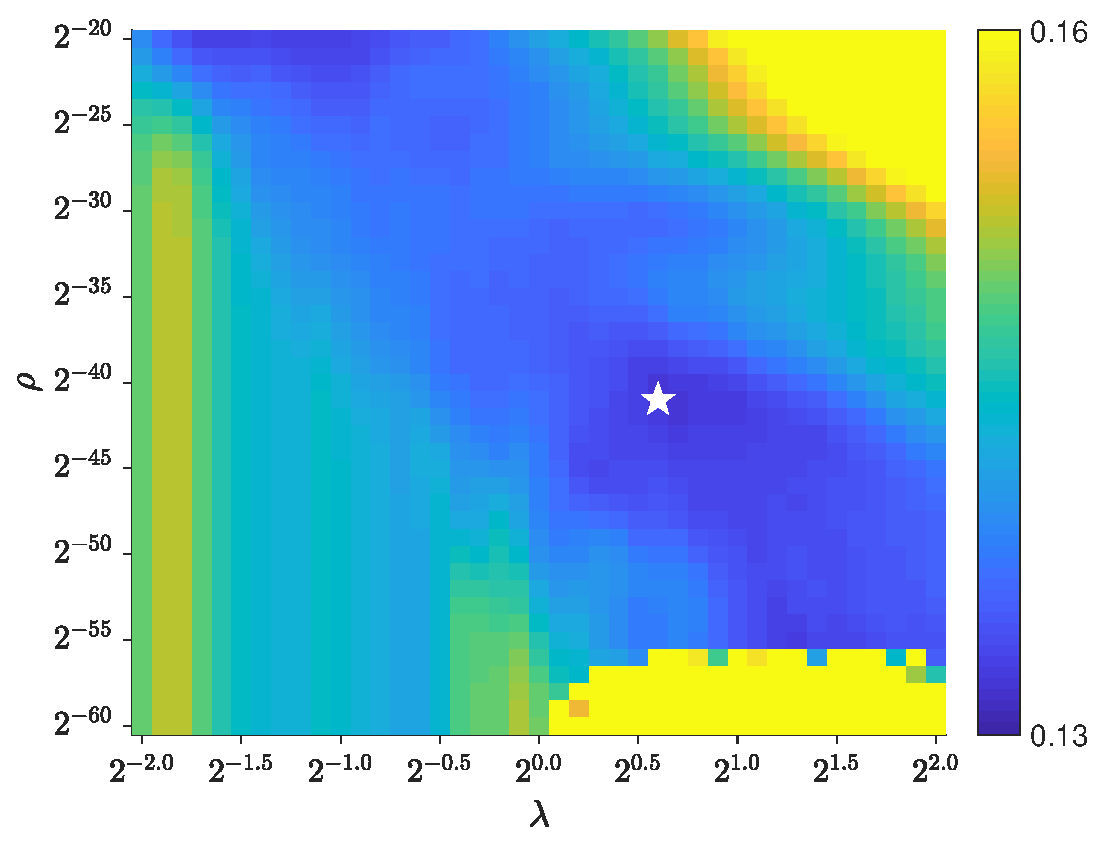
\includegraphics [width=\textwidth] {%
		tune/nrmse,w-t12.eps%
	}
	\caption{%
		Holdout criterion $\Psi\paren{\lambda,\rho}$
		versus Gaussian kernel bandwidth scaling parameter $\lambda$ 
		and regularization parameter $\rho$.
		Each pixel is the weighted normalized root mean squared error
  	of a candidate PERK estimator,
		where the empirical mean over $10^5$ test points
		approximates an expectation 
		with respect to training prior distribution $\dist{\bmx,\bmnu}$
		and the weighting places emphasis
		on good $\To,\Tt$ estimation performance.
		A white star marks the minimizer
		$\paren{\est{\lambda},\est{\rho}} \gets \paren{2^{0.6},2^{-41}}$.
	}
	\label{fig:perk,holdout}
\end{figure}

Fig.~\ref{fig:perk,holdout} plots $\costa{\lambda,\rho}$
for $T \gets 10^5$ test points 
and $\bmW \gets \diag{\brac{0,0.5,0.5}\tpose}$
selected to place equal emphasis 
on $\To,\Tt$ estimation.
We chose our fine grid search range
using a preliminary coarse grid search
spanning a much wider range
of $\paren{\lambda,\rho}$ values.
Overall, 
we observe a broad range of $\paren{\lambda,\rho}$ values
that yield similar cost function values.
Holdout cost $\costa{\lambda,\rho}$ gracefully increases
with larger $\paren{\lambda,\rho}$ values
due to under-fitting.
For very small $\rho$ values,
$\costa{\lambda,\rho}$ can be large
because poorly conditioned matrix inversions
cause machine imprecision 
to dominate estimation error.
In all simulations and experiments,
we fixed free model parameters
to the minimizer 
$\paren{\est{\lambda},\est{\rho}} \gets \paren{2^{0.6},2^{-41}}$,
indicated by a white star.

%%%%%%%%%%%%%%%%%%%%%%%%%%%%%%%%%%%%%%%%%%%%%%%%%%%
\subsubsection{Evaluation}
\label{sss,perk,exp,meth,eval}

We evaluated PERK latent parameter estimates
against maximum-likelihood (ML) estimates
computed via two well-suited algorithms
that we describe here in turn.
We first implemented a grid search estimator
accelerated by the variable projection method (VPM) \cite{golub:03:snl},
a popular technique 
that has been used
in many QMRI algorithms and applications
(see \eg 
\cite{%
	gong:92:aft,%
	haldar:07:mle,%
	hernando:08:jeo,%
	barral:10:arm,%
	ma:13:mrf,%
	mcgivney:14:scf,%
	trzasko:13:etf,%
	zhao:15:amp,%
	zhao:16:mlr,%
	he:16:ahd,%
	nataraj:17:oms%
}%
).
Following \cite{nataraj:17:oms},
we clustered flip angle scaling map voxels into 20 clusters
via $k$-means$++$ \cite{arthur:07:kmt}
and used each of the 20 cluster means
along with 
500 $\To$ and $\Tt$ values
logarithmically spaced 
between $\paren{{10}^{1.5}, {10}^{3.5}}$ 
and $\paren{{10}^{0.5},{10}^{3}}$
to compute 20 dictionaries,
each consisting of $250,000$ signal vectors
(fewer clusters introduced noticeable errors
in experiments).
Iterating over clusters,
we generated each cluster's dictionary
and applied VPM and grid search
over magnitude image data voxels
assigned to that cluster.

We also compared PERK 
to iterative ML optimization
via a preconditioned variant 
of the classical gradient projection method (PGPM) \cite{rosen:60:tgp}.
We designed the preconditioner 
as the inverse 
of a positive definite diagonal majorizer
of the negative log-likelihood cost function's Hessian matrix,
updated for the first five iterations
and fixed thereafter. 
We employed a diagonal preconditioner
to retain the linear convergence rate guarantees
of GPM \cite{bertsekas:82:pnm}
yet accelerate practical performance.
We initialized PGPM 
via conventional method-of-moments estimators
of $\mzero,\To$ from 2 SPGR scans \cite{gupta:77:anl}
and $\Tt$ from 1 DESS scan \cite{bruder:88:ans}
(the method-of-moments $\Tt$ estimator is strongly biased). 
We used the \matlab Symbolic Toolbox
to generate cumbersome but analytical expressions
for the gradient and Hessian 
of the magnitude SPGR and DESS signal models.
At each PGPM iteration,
we used these expressions
to compute a preconditioned descent direction,
update the iterate,
and project each voxel's $\To$ and $\Tt$ iterate
to lie within $[100,3000]$ms and $[10,700]$ms,
respectively.
We continued iterations
until the convergence criterion
\begin{align}
	\frob{\inv{\bmOmega}\paren{\iter{\bmX}{i}-\iter{\bmX}{i-1}}} 
		< 10^{-7} \frob{\inv{\bmOmega}\paren{\iter{\bmX}{i-1}}}
	\label{eq:perk,conv-crit}
\end{align}
was satisfied,
where $\bmX$ collects latent parameter voxels 
in its columns,
$\iter{\paren{\cdot}}{i}$ denotes the $i$th iterate,
$\bmOmega := \diag{\med{\iter{\bmX}{0}}}$ 
is a fixed latent parameter weighting matrix,
and $\med{\cdot}$ takes the median
across the columns of its argument.

To ensure monotone local convergence in cost,
we implemented PGPM to include 
a simple step-halving line search at each iteration.
In early experiments however,
we observed even in simulation 
and even with preconditioning
that attempting to update all voxels simultaneously 
using a single line search 
resulted in large errors
due to excessive step-halving 
and subsequent early termination of iterations. 
To circumvent separate line searches for every voxel,
we first clustered latent parameter initializations
and flip angle scaling map voxels into 50 clusters
and then ran PGPM separately on each cluster
(fewer clusters reintroduced early stopping).

We performed all simulations and experiments
running \matlab R2013a
on a 3.5GHz desktop computer
equipped with 32GB RAM. 
Because our experiments use a single slice of image data,
we report PERK training and testing times separately 
and note that only the latter time 
would scale linearly with the number of voxels
(the former would scale negligibly 
due only to online model selection).
In the interest of reproducible research,
code and data will be freely available
at \url{https://gitlab.eecs.umich.edu/fessler/qmri}.

%%%%%%%%%%%%%%%%%%%%%%%%%%%%%%%%%%%%%%%%%%%%%%%%%%%
\subsection{Numerical Simulations}
\label{ss,perk,exp,sim}

We assigned typical $\To,\Tt$ values 
in white matter (WM) and grey matter (GM) at 3T
\cite{wansapura:99:nrt}
to the 81st slice 
of the BrainWeb digital phantom
\cite{collins:98:dac}
to produce ground truth $\mzero,\To,\Tt$ maps.
We simulated $217 \times 181$
noiseless single-coil SPGR and DESS image data,
modeling (and then assuming as known)
$20\%$ flip angle spatial variation.
We corrupted noiseless datasets
with additive complex Gaussian noise
to yield noisy complex datasets 
with SNR ranging from 94-154 in WM and 82-154 in GM,
where SNR is defined
\begin{align}
	\snr{\bmyt,\bmepst} := \norm{\bmyt}_2/\norm{\bmepst}_2
	\label{eq:perk,snr}
\end{align}
for image data voxels $\bmyt$ and noise voxels $\bmepst$
corresponding to a region of interest (ROI)
within a single SPGR/DESS dataset.
We estimated $\mzero,\To,\Tt$ 
from noisy magnitude images and known $\kappa$ maps
using VPM, PGPM, and PERK.
VPM took 791s;
PGPM took 1821s;
and 
PERK training and testing respectively took 3.6s and 1.5s.

\begin{figure}[!ht]
	\centering
	\subfigure{%
		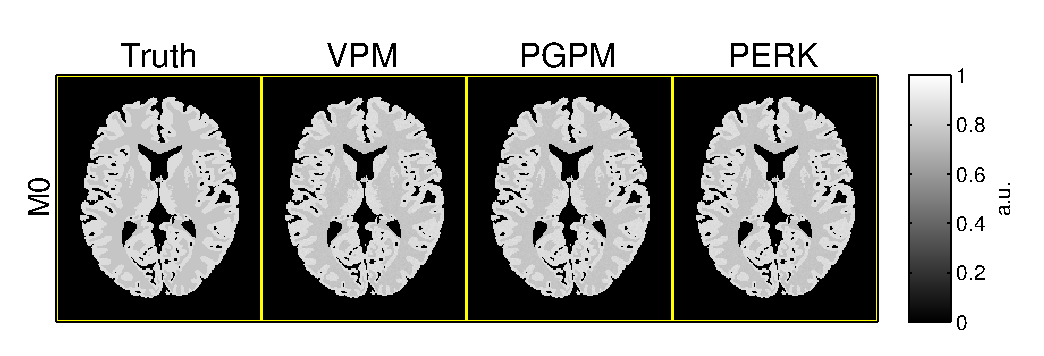
\includegraphics [width=0.99\textwidth] {%
			sim/sp2de1,sl-81,m0,im,gray.eps%
		}
		\label{fig:perk,sim,m0,im,gray}
	}
	\hspace{0cm}
	\subfigure{%
		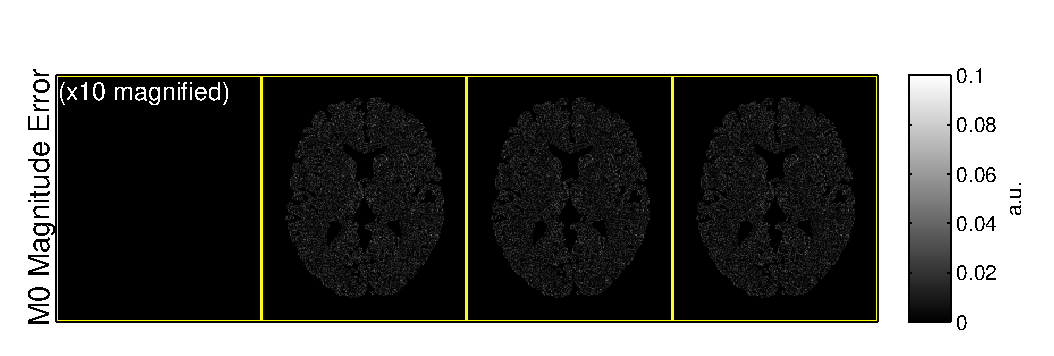
\includegraphics [width=\textwidth,trim=0 0 0 25,clip] {%
			sim/sp2de1,sl-81,m0,err,gray.eps%
		}
		\label{fig:perk,sim,m0,err,gray}
	}
	\caption{%
		$\mzero$ VPM, PGPM, and PERK estimates
		and corresponding error images,
		in simulation.
		Magnitude error images are $10\times$ magnified.
		Voxels not assigned WM- or GM-like relaxation times
		are masked out in post-processing for display.
		Difference images demonstrate
		that all three $\mzero$ estimates
		exhibit low estimation error.
		Table~\ref{tab:perk,sim} presents
		corresponding sample statistics.
	}
	\label{fig:perk,sim,m0}
\end{figure}
	
\begin{figure}[!ht]
	\centering
	\subfigure{%
		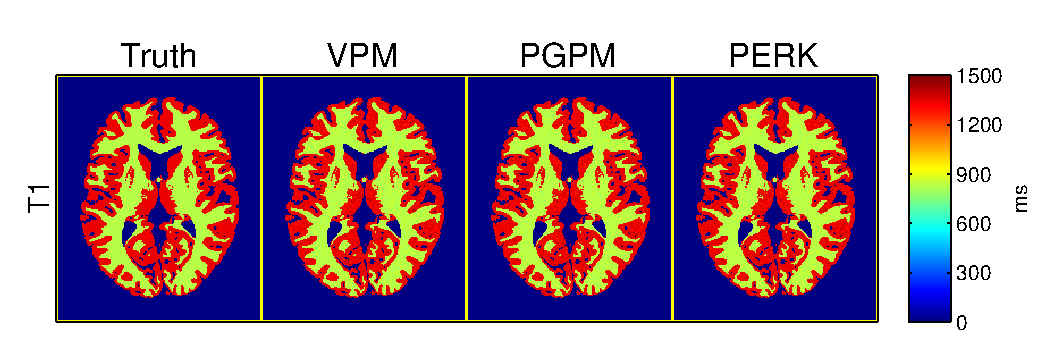
\includegraphics [width=\textwidth] {%
			sim/sp2de1,sl-81,t1,im,jet.eps%
		}
		\label{fig:perk,sim,t1,im,jet}
	}
	\hspace{0cm}
	\subfigure{%
		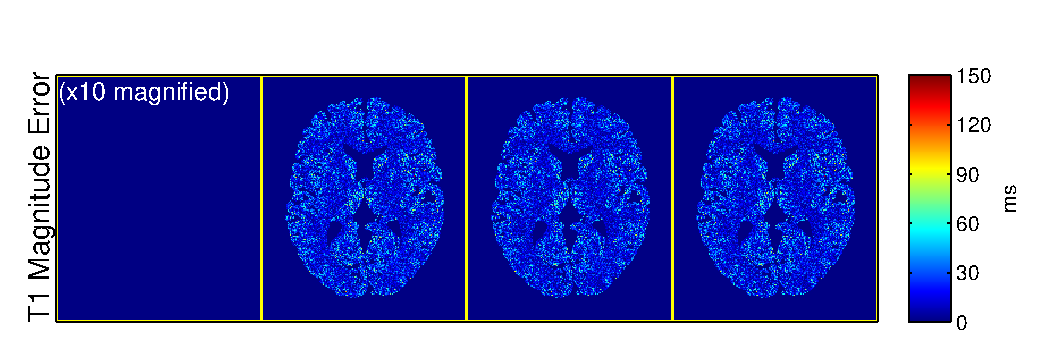
\includegraphics [width=0.99\textwidth,trim=0 0 0 25,clip] {%
			sim/sp2de1,sl-81,t1,err,jet.eps%
		}
		\label{fig:perk,sim,t1,err,jet}
	}
	\caption{%
		$\To$	VPM, PGPM, and PERK estimates
		and corresponding error images,
		in simulation.
		Magnitude error images are $10\times$ magnified.
		Voxels not assigned WM- or GM-like relaxation times
		are masked out in post-processing for display.
		Difference images demonstrate
		that all three $\To$ estimates
		exhibit low estimation error.
		Table~\ref{tab:perk,sim} presents
		corresponding sample statistics.
	}
	\label{fig:perk,sim,t1}
\end{figure}

\begin{figure}[!ht]
	\centering
	\subfigure{%
		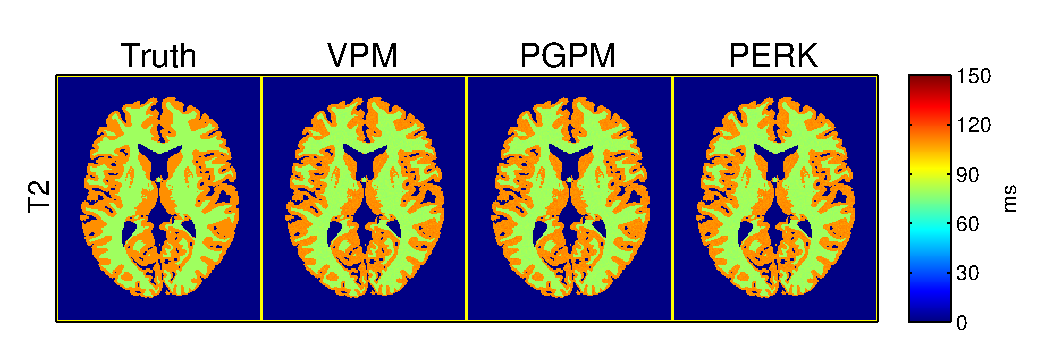
\includegraphics [width=\textwidth] {%
			sim/sp2de1,sl-81,t2,im,jet.eps%
		}
		\label{fig:perk,sim,t2,im,jet}
	}
	\hspace{0cm}
	\subfigure{%
		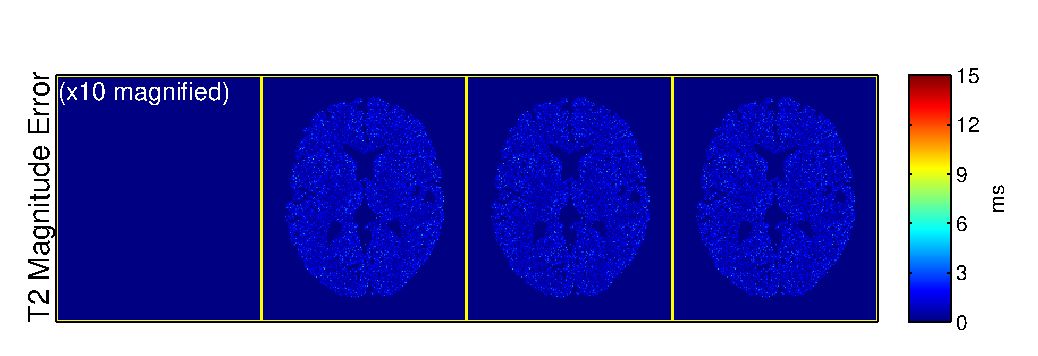
\includegraphics [width=0.99\textwidth,trim=0 0 0 25,clip] {%
			sim/sp2de1,sl-81,t2,err,jet.eps%
		}
		\label{fig:perk,sim,t2,err,jet}
	}
	\caption{%
		$\Tt$ VPM, PGPM, and PERK estimates
		and corresponding error images,
		in simulation.
		Magnitude error images are $10\times$ magnified.
		Voxels not assigned WM- or GM-like relaxation times
		are masked out in post-processing for display.
		Difference images demonstrate
		that all three $\To$ estimates
		exhibit low estimation error.
		Table~\ref{tab:perk,sim} presents
		corresponding sample statistics.
	}
	\label{fig:perk,sim,t2}
\end{figure}

Figs.~\ref{fig:perk,sim,m0}, \ref{fig:perk,sim,t1}, and \ref{fig:perk,sim,t2}
compare VPM, PGPM, and PERK estimates
of $\mzero$, $\To$, $\Tt$ respectively,
alongside $10\times$ magnified absolute difference images 
with respect to the ground truth.
Voxels not assigned WM- or GM-like relaxation times
are masked out in post-processing for display.
Difference images demonstrate
that within WM- and GM-like voxels,
all three methods exhibit low estimation error.

\begin{table}[!ht]
	\footnotesize
	\centering
	\begin{tabular}{c | r | r r r}
		\hline
		\hline
								& Truth 	& VPM 													
													& PGPM 																	& PERK \\
		\hline
		WM $\mzero$	& $0.77$	& \mnstd{0.7700}{0.00919} $(0.0092)$ 
													& \mnstd{0.76999}{0.00871} $(0.00871)$ 	& \mnstd{0.77002}{0.00873} $(0.00873)$ \\
		GM $\mzero$	& $0.86$	& \mnstd{0.8601}{0.01192} $(0.0119)$
													& \mnstd{0.8600}{0.01142} $(0.0114)$ 		& \mnstd{0.8613}{0.01147} $(0.0133)$ \\
		\hline
		WM $\To$ 		& $832$ 	& \mnstd{832.1}{17.2} $(17.2)$	
													& \mnstd{832.1}{16.2} $(16.2)$ 					& \mnstd{833.0}{16.5} $(16.5)$ \\
		GM $\To$ 		& $1331$ 	& \mnstd{1331.5}{31.1} $(31.1)$ 
													& \mnstd{1331.2}{29.7} $(29.7)$ 				& \mnstd{1332.1}{30.4} $(30.4)$ \\ 
		\hline
		WM $\Tt$ 		& $79.6$	& \mnstd{79.61}{0.988} $(0.988)$
													& \mnstd{79.60}{0.952} $(0.952)$ 				& \mnstd{79.46}{0.978} $(0.989)$ \\
		GM $\Tt$ 		& $110.$ 	& \mnstd{110.02}{1.40} $(1.40)$
													& \mnstd{110.02}{1.35} $(1.35)$ 				& \mnstd{109.91}{1.35} $(1.35)$ \\
    \hline
    \hline
  \end{tabular}
  \caption{%
  	Sample means $\pm$ sample standard deviations (RMSEs)
		of VPM, PGPM, and PERK $\mzero,\To,\Tt$ estimates,
		computed in simulation
		over $7810$ WM-like and $9162$ GM-like voxels.
		Each sample statistic is rounded off
		to the highest place value
		of its (unreported) standard error,
		computed via formulas in \cite{ahn:03:seo}.
		$\mzero$ values are unitless.
		$\To,\Tt$ values are in milliseconds.
		Figs.~\ref{fig:perk,sim,m0}, \ref{fig:perk,sim,t1}, and \ref{fig:perk,sim,t2}
		present corresponding images.
	}
	\label{tab:perk,sim}
\end{table}

Table~\ref{tab:perk,sim} compares sample statistics
of VPM, PGPM, and PERK $\mzero,\To,\Tt$ estimates,
computed over $7810$ WM-like and $9162$ GM-like voxels.
Overall,
all three methods achieve excellent performance.
PERK estimates are slightly more precise 
but slightly less accurate 
than gold-standard VPM estimates. 
Results suggest that 
at least in WM- and GM-like voxels,
PGPM is capable of descending the ML cost 
towards a desirable solution;
in fact, PGPM achieves slightly better precision
than either VPM or PERK.
All three methods exhibit comparable 
root mean squared errors (RMSEs).

%%%%%%%%%%%%%%%%%%%%%%%%%%%%%%%%%%%%%%%%%%%%%%%%%%%
\subsection{Phantom Experiments}
\label{ss,perk,exp,phant}

\begin{figure}[!t]
	\centering
	\begin{minipage}{\textwidth}
  	\subfigure{%
  		\includegraphics [width=0.96\textwidth] {%
  			hpd-tight/sp2de1,sl-6,m0,im-gray.eps%
  		}
  		\label{fig:perk,hpd-tight,m0,im-gray}
  	}
  	\hspace{0cm}
  	\subfigure{%
  		\includegraphics [width=0.982\textwidth,trim=0 0 0 25,clip] {%
  			hpd-tight/sp2de1,sl-6,t1,im-jet.eps%
  		}
  		\label{fig:perk,hpd-tight,t1,im-jet}
  	}
  	\hspace{0cm}
  	\subfigure{%
  		\includegraphics [width=0.97\textwidth,trim=0 0 0 25,clip] {%
  			hpd-tight/sp2de1,sl-6,t2,im-jet.eps%
  		}
  		\label{fig:perk,hpd-tight,t2,im-jet}
  	}
	\end{minipage}
	\caption{%
		VPM, PGPM, and PERK $\mzero,\To,\Tt$ estimates 
		in a quantitative phantom.
		Vials are enumerated and highlighted
		to correspond with markers and colored boxes
		in Fig.~\ref{fig:perk,hpd-tight,plot}.
		PERK has only been trained 
		to accurately estimate within vials 4-8;
		within these vials,
		VPM, PGPM, and PERK estimates 
		appear visually similar.
	}
	\label{fig:perk,hpd-tight}
\end{figure}

\begin{figure*}[!t]
	\centering
	\subfigure{%
		\includegraphics [width=0.47\textwidth]{%
			hpd-tight/sp2de1,sl-6,t1,plot%
		}
		\label{fig:perk,hpd-tight,t1,plot}
	}
	\hspace{0.3cm}
	\subfigure{%
		\includegraphics [width=0.47\textwidth] {%
			hpd-tight/sp2de1,sl-6,t2,plot%
		}
		\label{fig:perk,hpd-tight,t2,plot}
	}
	\vspace{0.3cm}
	\begin{tabular}{c || r | r r r}
		\hline
		\hline
		 					& NMR										& VPM 							& PGPM									& PERK \\
		\hline
		V4 $\To$	& \mnstd{1604}{7.2} 		& \mnstd{1645}{48} 	& \mnstd{1649}{48}			& \mnstd{1626}{46} 	\\        
    V5 $\To$	& \mnstd{1332}{0.8} 		& \mnstd{1335}{61} 	& \mnstd{1331}{41}			& \mnstd{1332}{40.} \\        
    V6 $\To$	& \mnstd{1044}{3.2} 		& \mnstd{1055}{28} 	& \mnstd{1060.}{29}			& \mnstd{1061}{29} 	\\        
    V7 $\To$	& \mnstd{801.7}{1.70}		& \mnstd{834}{21} 	& \mnstd{840.}{23}			& \mnstd{839}{23} 	\\         
    V8 $\To$	& \mnstd{608.6}{1.03} 	& \mnstd{627}{25} 	& \mnstd{623}{12}				& \mnstd{620.}{13} 	\\    
		\hline
		\hline
		V4 $\Tt$	& \mnstd{190.94}{0.011}	&	\mnstd{194}{5.5}	& \mnstd{192.4}{5.2}		& \mnstd{192.5}{4.9}\\    
    V5 $\Tt$	& \mnstd{133.27}{0.073} &	\mnstd{131.2}{5.3}& \mnstd{131}{5.5} 			& \mnstd{131}{5.5}  \\       
    V6 $\Tt$	& \mnstd{96.89}{0.049}  &	\mnstd{90.8}{3.5} & \mnstd{90.8}{3.5}			& \mnstd{90.9}{3.5} \\         
    V7 $\Tt$	& \mnstd{64.07}{0.034}  &	\mnstd{64.6}{2.2} & \mnstd{64.5}{2.1} 		& \mnstd{65.0}{2.1} \\        
    V8 $\Tt$	& \mnstd{46.42}{0.014}  &	\mnstd{46.4}{1.5} & \mnstd{46.4}{1.5} 		& \mnstd{46.1}{1.5} \\   
		\hline
		\hline
	\end{tabular}
	\caption{%
		Phantom sample statistics
		of VPM, PGPM, and PERK $\To,\Tt$ estimates
		and NIST NMR reference measurements \cite{keenan:16:msm}.
		Plot markers and error bars indicate sample means
		and sample standard deviations
		computed over ROIs
		within the 14 vials
		labeled and color-coded 
		in Fig.~\ref{fig:perk,hpd-tight}.
		Yellow box boundaries 
		indicate projections
		of the PERK sampling distribution's support $\supp{\dist{\bmx,\bmnu}}$.
		Missing markers lie outside axis limits.
		Corresponding tables replicate 
		sample means $\pm$ sample standard deviations
		for vials within $\supp{\dist{\bmx,\bmnu}}$.
		Each value is rounded off
		to the highest place value 
		of its (unreported) standard error,
		computed via formulas in \cite{ahn:03:seo}.
		`V\#' indicates vial numbers.
		All values are reported in milliseconds.
		Within $\supp{\dist{\bmx,\bmnu}}$, 
		VPM, PGPM, and PERK estimates agree excellently 
		with each other
		and reasonably with NMR measurements.
	}
	\label{fig:perk,hpd-tight,plot}
\end{figure*}		 

Phantom experiments used datasets 
from fast coronal scans
of a High Precision Devices\regis MR system phantom $\Tt$ array
acquired on a 3T GE Discovery\tmark scanner
with an 8-channel receive head array.
This acquisition consisted of: 
two SPGR scans 
with $5,15^\circ$ flip angles
and $12.2,12.2$ms repetition times;
one DESS scan 
with $30^\circ$ flip angle
and $17.5$ms repetition time;
and two Bloch-Siegert (BS) scans \cite{sacolick:10:bmb}
(for separate flip angle scaling estimation).
Nominal flip angles were achieved 
by scaling a 2cm slab-selective Shinnar-Le Roux RF pulse \cite{pauly:91:prf}
of duration 1.28ms and time-bandwidth product 4.
All scans collected fully-sampled 3D Cartesian data
using 4.67ms echo times
with a $256\times256\times8$ matrix
over a $24\times24\times4$cm$^3$ field of view. 
Scan time totaled 3m17s. 
The scan room temperature was recorded as $293$K
at the beginning of the exam. 
Further acquisition details are in \cite{nataraj:17:oms}.

For each SPGR, DESS, and BS dataset, 
we reconstructed raw coil images via 3D Fourier transform
and subsequently processed only one image slice
centered within the excitation slab.
We combined SPGR and DESS coil images 
using a natural extension of \cite{ying:07:jir}
to the case of multiple datasets.
We similarly (but separately) combined BS coil images
and estimated $\kappa$ maps
by normalizing and calibrating
regularized transmit field estimates \cite{sun:14:reo}
from complex coil-combined BS images.
We estimated $\mzero,\To,\Tt$
from magnitude SPGR/DESS images and $\kappa$ maps
using VPM, PGPM, and PERK.
VPM took 928s;
PGPM took 1257s; 
and PERK training and testing
respectively took 4.2s and 1.9s.

Fig.~\ref{fig:perk,hpd-tight} compares
VPM, PGPM, and PERK $\mzero,\To,\Tt$ estimates.
Vials are enumerated in descending $\To,\Tt$ order.
Vials whose $\To,\Tt$ values
are within sampling distribution support $\supp{\dist{\bmx,\bmnu}}$
(as measured by NIST NMR reference measurements \cite{keenan:16:msm})
have labels highlighted
with yellow numbers.
Here, 
$\supp{\dist{\bmx,\bmnu}}$ was chosen 
to reflect the ranges of latent parameter values
for which the SPGR/DESS scan parameters 
were optimized in \cite{nataraj:17:oms}.
Circular ROIs are selected well away from vial encasings
and correspond with sample statistics 
presented in Fig.~\ref{fig:perk,hpd-tight,plot}.                                                                                                                                                                                 
Distilled water surrounds the encased vials.
Within the highlighted vials of interest,
VPM, PGPM, and PERK estimates 
appear visually similar.

Fig.~\ref{fig:perk,hpd-tight,plot} compares
sample means and sample standard deviations
computed within ROIs 
of VPM, PGPM, and PERK $\To,\Tt$ estimates
against nuclear magnetic resonance (NMR) reference measurements 
reported at 293.00K
from the National Institute 
for Standards of Technology (NIST) \cite{keenan:16:msm}.
Yellow box boundaries indicate projections
of the PERK sampling distribution's support $\supp{\dist{\bmx,\bmnu}}$.
ROI labels correspond with vial markers
depicted in Fig.~\ref{fig:perk,hpd-tight}.
Within $\supp{\dist{\bmx,\bmnu}}$,
corresponding tables demonstrate
that VPM, PGPM, and PERK estimates agree excellently 
with each other 
and reasonably with NMR measurements.
We do not expect good PERK performance
outside $\supp{\dist{\bmx,\bmnu}}$ 
and indeed observe 
poor ability to extrapolate.
As discussed in Subsection~\ref{sss,perk,pract,mod,dist}
and demonstrated in Subsection~\ref{ss,perk,robust,dist},
expanding $\supp{\dist{\bmx,\bmnu}}$
well beyond the acquisition design 
parameter range of interest
can reduce PERK performance
for typical $\To,\Tt$ WM and GM values.

%%%%%%%%%%%%%%%%%%%%%%%%%%%%%%%%%%%%%%%%%%%%%%%%%%%
\subsection{\Invivo Experiments}
\label{ss,perk,exp,invivo}

\Invivo experiments used datasets
from axial scans of a healthy volunteer
acquired with a 32-channel Nova Medical\regis receive head array.
To address bulk motion between scans,
we rigidly registered coil-combined images 
to a reference
before parameter estimation.
All other data acquisition, 
image reconstruction, 
and parameter estimation details
are the same as in phantom experiments
(acquisition and reconstruction details 
are reported in \cite{nataraj:17:oms}).
VPM took 838s;
PGPM took 2178s;
and PERK training and testing
took 4.2s and 1.6s.

\begin{figure*}[!ht]
	\centering
	\begin{minipage}{\textwidth}
  	\subfigure{%
  		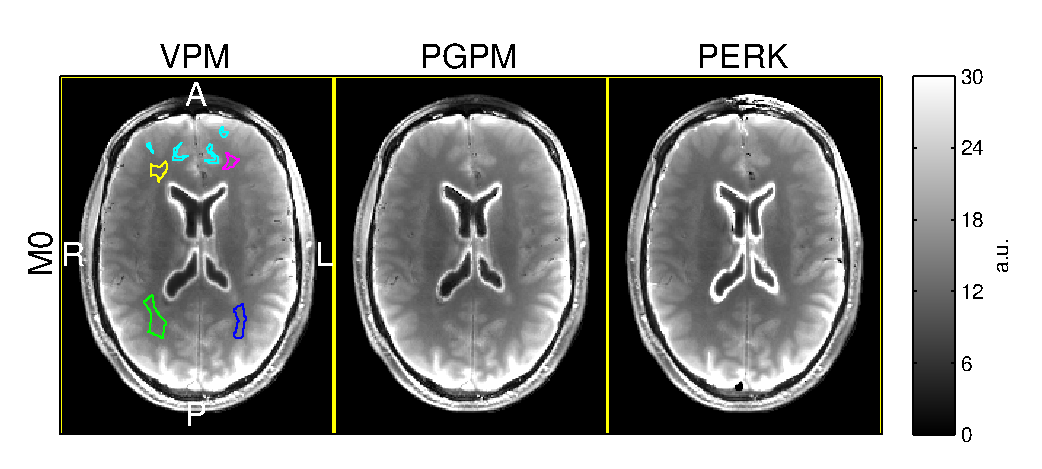
\includegraphics [width=0.96\textwidth,trim=0 0 0 10,clip] {%
  			brain/sp2de1,sl-5,m0,im-gray.eps%
  		}%
  		\label{fig:perk,brain,m0,im-gray}
  	}%
  	\hspace{0cm}
  	\subfigure{%
  		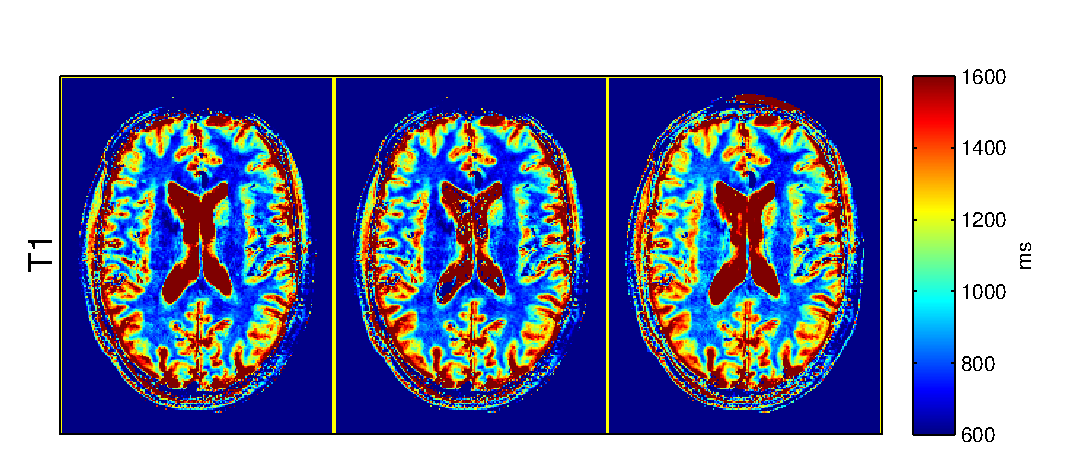
\includegraphics [width=0.982\textwidth,trim=0 0 0 20,clip] {%
  			brain/sp2de1,sl-5,t1,im-jet.eps%
  		}
  		\label{fig:perk,brain,t1,im-jet}
  	}%
  	\hspace{0cm}
  	\subfigure{%
  		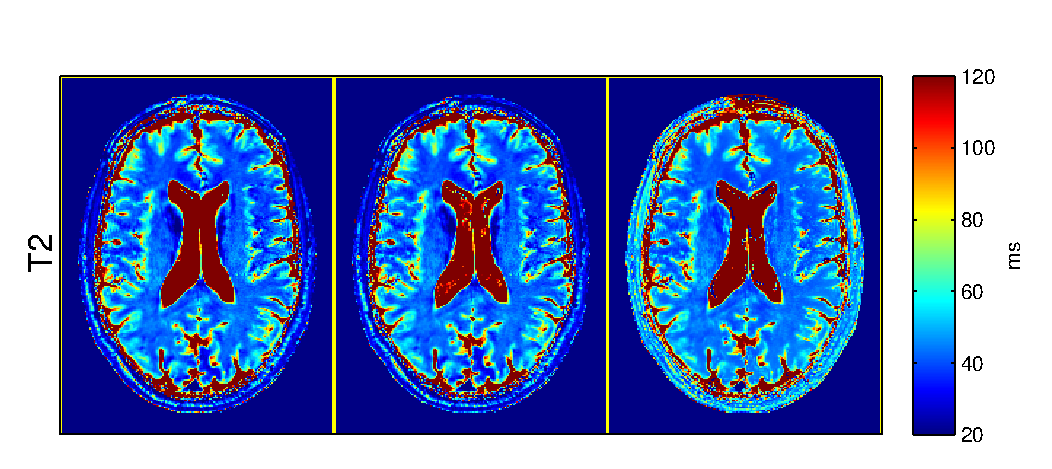
\includegraphics [width=0.97\textwidth,trim=0 0 0 20,clip] {%
  			brain/sp2de1,sl-5,t2,im-jet.eps%
  		}%
  		\label{fig:perk,brain,t2,im-jet}
  	}%
	\end{minipage}
	\caption{%
		VPM, PGPM and PERK estimates
		of $\mzero,\To,\Tt$ 
		in the brain of a healthy volunteer.
		Separate WM ROIs are distinguished
		by anterior/posterior (A/P)
		and right/left (R/L) directions.
		Four small anterior cortical GM polygons
		are pooled into a single GM ROI.
		Images are cropped in post-processing 
		for display.
	}
	\label{fig:perk,brain}
\end{figure*}

\begin{table}[!ht]
	\centering
	\begin{tabular}{r | c | r r r}
		\hline
		\hline
			& ROI 		& VPM 							& PGPM 							& PERK 									\\
		\hline
		\multirow{5}{*}{$\To$}
			& \AR WM 	& \mnstd{778}{28}		& \mnstd{779}{27}		& \mnstd{832}{31} 			\\
      & \AL WM 	& \mnstd{731}{37}   & \mnstd{713}{33}		& \mnstd{725}{41}				\\
      & \PR WM 	& \mnstd{805}{52}   & \mnstd{796}{51}		& \mnstd{831}{51}				\\
      & \PL WM 	& \mnstd{789}{40}   & \mnstd{788}{38} 	& \mnstd{815}{42}				\\
      & \A 	GM 	& \mnstd{1120}{180} & \mnstd{1120}{180}	& \mnstd{1150}{170.}		\\
    \hline
    \multirow{5}{*}{$\Tt$}
      & \AR WM 	&	\mnstd{40.0}{1.29}& \mnstd{40.0}{1.27}& \mnstd{41.18}{0.94} 	\\
      & \AL WM 	& \mnstd{39.7}{1.7} & \mnstd{39.7}{1.7}	& \mnstd{41.3}{1.02}		\\
      & \PR WM	& \mnstd{43.0}{2.7} & \mnstd{43.0}{2.7} & \mnstd{43.7}{2.6}			\\
      & \PL WM 	&	\mnstd{43.0}{1.8} &	\mnstd{43.0}{1.8} & \mnstd{43.5}{1.36}		\\
      & \A 	GM	& \mnstd{53.5}{11.8}&	\mnstd{53.4}{11.7}& \mnstd{53.3}{11.6}		\\
   	\hline
		\hline
	\end{tabular}
	\caption{%
		\Invivo sample means $\pm$ sample standard deviations
		of VPM, PGPM, and PERK $\To,\Tt$ estimates,
		computed over color-coded ROIs
		indicated in Fig.~\ref{fig:perk,brain}.
		Each value is rounded off 
		to the highest place value
		of its (unreported) standard error,
		computed via formulas in \cite{ahn:03:seo}.
		All values are in milliseconds.
	}
	\label{tab:perk,brain}
\end{table}

Fig.~\ref{fig:perk,brain} compares 
VPM, PGPM, and PERK $\mzero,\To,\Tt$ estimates.
The PERK $\mzero$ estimate appears smoothed
(although no spatial regularization was used)
but is otherwise very similar
to the VPM and PGPM $\mzero$ estimates.
Narrow display ranges emphasize
that VPM, PGPM, and PERK $\To,\Tt$ estimates 
discern cortical WM/GM boundaries similarly,
though PERK $\To$ estimates are noticeably highest
in some WM regions.
VPM, PGPM, and PERK $\Tt$ estimates are nearly indistinguishable 
in lateral regions
but disagree somewhat 
in medial regions close 
to cerebrospinal fluid (CSF).
We neither expect nor observe reasonable PERK performance
in voxels containing CSF.

Table~\ref{tab:perk,brain} summarizes sample statistics
of VPM, PGPM, and PERK $\To,\Tt$ estimates,
computed over four separate WM ROIs 
containing $96$, $69$, $224$, and $148$ voxels
and one pooled cortical anterior GM ROI 
containing $156$ voxels.
Overall,
VPM, PGPM, and PERK $\To,\Tt$ estimates are comparable.
$\To$ estimates in GM
and $\Tt$ estimates in WM/GM
do not differ significantly.
PERK $\To$ estimates are significantly higher
than VPM and PGPM $\To$ estimates 
in one WM ROI;
however,
all $\To$ estimates 
are well within the range 
of typical literature measurements at 3T 
(see \eg \cite{wansapura:99:nrt, stanisz:05:ttr}).

%%%%%%%%%%%%%%%%%%%%%%%%%%%%%%%%%%%%%%%%%%%%%%%%%%%
\section{Robustness Studies}
\label{s,perk,robust}
%%%%%%%%%%%%%%%%%%%%%%%%%%%%%%%%%%%%%%%%%%%%%%%%%%%

This section investigates PERK robustness
to two types of non-idealities
that may be encountered 
in other applications.
Subsection~\ref{ss,perk,robust,noise} 
studies PERK performance sensitivity
to mismatch between training and testing noise variance.
Subsection~\ref{ss,perk,robust,dist}
studies PERK performance degradation
when trained 
with latent parameter distributions
that have wider support
than the parameter ranges
used for optimizing the scan design
in \cite{nataraj:17:oms}.

%%%%%%%%%%%%%%%%%%%%%%%%%%%%%%%%%%%%%%%%%%%%%%%%%%%
\subsection{Mismatch in Training vs. Testing Noise Statistics}
\label{ss,perk,robust,noise}

\begin{figure}[!t]
	\centering
	\subfigure{%
		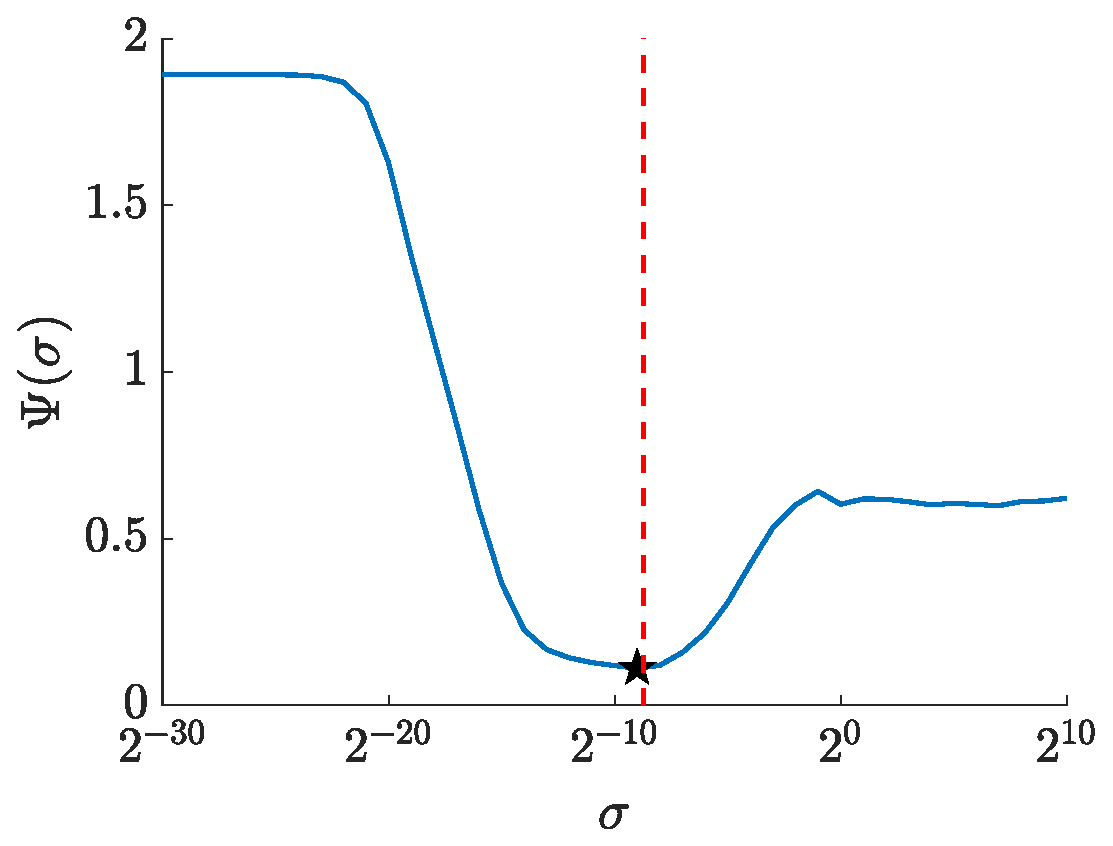
\includegraphics [width=0.47\textwidth] {%
			tune/robust,broad,w-t12.eps%
		}
		\label{fig:perk,robust,broad}
	}
	\hspace{0cm}
	\subfigure{%
		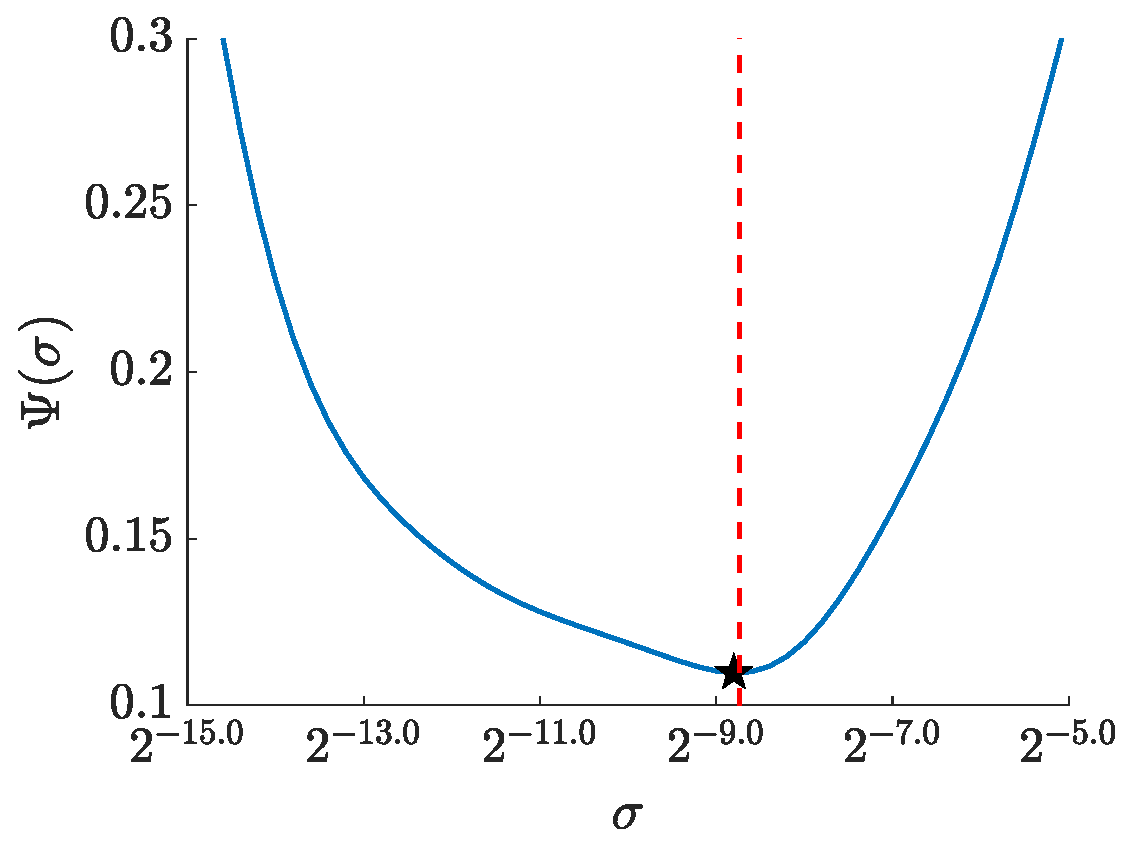
\includegraphics [width=0.47\textwidth] {%
			tune/robust,tight,w-t12.eps%
		}
		\label{fig:perk,robust,tight}
	}
	\caption{%
		Performance criterion $\costa{\sigma}$
		versus PERK training noise standard deviation $\sigma$,
		over two different scales.
		Similar to Fig.~\ref{fig:perk,holdout},
		each point on the blue curve
		is the weighted normalized root mean squared error
		of a separately trained PERK estimator.
		In each subplot,
		a black star marks 
		the performance criterion minimizer
		$\est{\sigma} \gets 2^{-8.8}$
		while a dashed red line
		marks the (latent) test data noise standard deviation 
		$\sigma^\star \gets 2^{-8.736}$.
		To within quantization error,
		PERK performs best 
		when trained with training data
		whose noise statistics 
		match test data noise statistics.
		Performance degradation as measured by $\cost$ 
		does not exceed $10\%$
		for $\sigma$ values within a factor of two
		of $\sigma^\star$.
		This result suggests 
		that PERK is somewhat robust
		to moderate misspecification of the noise level.
	}%
	\label{fig:perk,robust}
\end{figure}

To assess the importance
of training PERK
with appropriately noisy training data,
we investigated PERK's performance sensitivity
to the standard deviation $\sigma$
of the noise distribution 
from which noise realizations are drawn
to generate training data.
Instead of setting $\sigma$ online
as in other experiments,
here we fixed $\sigma$ offline
to one of many discretized values
spanning many orders of magnitude.
Otherwise as described 
in Subsection~\ref{ss,perk,exp,meth},
we trained a PERK estimator
for each $\sigma$ setting.
Similar to Subsection~\ref{sss,perk,exp,meth,holdout},
we tested each PERK estimator 
on a separate simulated dataset
consisting of $10^5$ samples 
from training prior distribution $\dist{\bmx,\bmnu}$.
We assessed performance sensitivity
by comparing evaluations $\costa{\sigma}$ 
of holdout cost \eqref{eq:perk,holdout}
at each $\sigma$ setting.
	
Fig.~\ref{fig:perk,robust} plots $\costa{\sigma}$
as $\sigma$ is varied 
over two different scales.
In each subplot,
a black star marks the minimizer 
$\hat{\sigma} \gets 2^{-8.8}$
while a dashed red line marks
the (latent) test data noise standard deviation 
$\sigma^\star \gets 2^{-8.736}$.
To within quantization error,
PERK performs best 
when trained with training data
whose noise statistics 
match test data noise statistics.
As measured by $\cost$, 
PERK performance degrades by at most $10\%$ 
for choices of $\sigma \in \brac{2^{-10.2},2^{-8}}$.
Results suggest
that for good PERK performance,
it is desirable
to set $\sigma$
to within about a factor of two
of the test data noise standard deviation $\sigma^\star$.
Nevertheless,
there is a zone near $\sigma^\star$
where PERK performance is reasonably similar,
indicating that PERK is somewhat robust
to some misspecification of the noise level.

%%%%%%%%%%%%%%%%%%%%%%%%%%%%%%%%%%%%%%%%%%%%%%%%%%%
\subsection{Mismatch in Scan Design vs. Sampling Distribution Support}
\label{ss,perk,robust,dist}

Although the SPGR/DESS acquisition
was optimized in \cite{nataraj:17:oms}
for a certain range of $\To,\Tt$ values,
it is interesting to investigate
how well PERK can perform 
outside that parameter range
if presented (simulated) training data
over a wider range of latent parameters.
It is also interesting to explore
whether using such a wider range 
of latent parameters for training
degrades performance
for the parameter range 
of primary interest.
Thus, 
we repeated the phantom experiment
described in Subsection~\ref{ss,perk,exp,phant}
except now using a PERK estimator
trained using a sampling prior distribution
with broader support.
We still assume a separable prior distribution
$\dist{\bmx,\bmnu} \gets \dist{\mzero}\dist{\To}\dist{\Tt}\dist{\kappa}$ 
(with $\dist{\mzero}$ and $\dist{\kappa}$ set as before)
but now set 
$\dist{\To} \gets \logunif{10^{1.5}, 10^{3.5}}$ 
and 
$\dist{\Tt} \gets \logunif{10^{0.5}, 10^{3.5}}$ 
to have wider supports.
These support endpoints 
now match the grid search support
used by the VPM.
All other training and testing details are unchanged from before.

\begin{figure*}[!t]
	\centering
	\subfigure{%
		\includegraphics [width=0.47\textwidth]{%
			hpd-broad/sp2de1,sl-6,t1,plot%
		}
		\label{fig:perk,hpd-broad,t1,plot}
	}
	\hspace{0.3cm}
	\subfigure{%
		\includegraphics [width=0.47\textwidth] {%
			hpd-broad/sp2de1,sl-6,t2,plot%
		}
		\label{fig:perk,hpd-broad,t2,plot}
	}
	\vspace{0.3cm}
	\begin{tabular}{c || r | r r r}
		\hline
		\hline
		 					& NMR										& VPM 							& PGPM 									& PERK 								\\
		\hline
		V4 $\To$	& \mnstd{1604}{7.2} 		& \mnstd{1645}{48} 	& \mnstd{1639}{48}			& \mnstd{1649}{51} 		\\        
    V5 $\To$	& \mnstd{1332}{0.8} 		& \mnstd{1335}{61} 	& \mnstd{1331}{41}			& \mnstd{1343}{40.} 	\\        
    V6 $\To$	& \mnstd{1044}{3.2} 		& \mnstd{1055}{28} 	& \mnstd{1060.}{29}			& \mnstd{1083}{32} 		\\        
    V7 $\To$	& \mnstd{801.7}{1.70}		& \mnstd{834}{21} 	& \mnstd{840.}{23}			& \mnstd{821}{25} 		\\         
    V8 $\To$	& \mnstd{608.6}{1.03} 	& \mnstd{627}{25} 	& \mnstd{623}{12}				& \mnstd{604}{18} 		\\  
		\hline
		\hline
		V4 $\Tt$	& \mnstd{190.94}{0.011}	&	\mnstd{194}{5.5}	& \mnstd{193.1}{5.2}		& \mnstd{197}{11}			\\    
    V5 $\Tt$	& \mnstd{133.27}{0.073} &	\mnstd{131.2}{5.3}& \mnstd{131}{5.5} 			& \mnstd{138}{8}  		\\       
    V6 $\Tt$	& \mnstd{96.89}{0.049}  &	\mnstd{90.8}{3.5} & \mnstd{90.8}{3.5}			& \mnstd{106.6}{3.6} 	\\         
    V7 $\Tt$	& \mnstd{64.07}{0.034}  &	\mnstd{64.6}{2.2} & \mnstd{64.5}{2.1} 		& \mnstd{89.2}{3.7} 	\\        
    V8 $\Tt$	& \mnstd{46.42}{0.014}  &	\mnstd{46.4}{1.5} & \mnstd{46.4}{1.5} 		& \mnstd{48.9}{4.6} 	\\
    \hline
    \hline      
	\end{tabular}
	\caption{%
		Phantom sample statistics
		of more aggressively trained 
		VPM, PGPM, and PERK $\To,\Tt$ estimates
		and NIST NMR reference measurements \cite{keenan:16:msm}.
		Unlike analogous results in Fig.~\ref{fig:perk,hpd-tight,plot},
		here the PERK estimator was trained
		with a sampling distribution
		whose support extended 
		well beyond the range of $\To,\Tt$ values
		for which the acquisition was optimized 
		in \cite{nataraj:17:oms}.
		Comparing to Fig.~\ref{fig:perk,hpd-tight,plot},
		we find that PERK estimator performance degrades 
		within the highlighted $\To,\Tt$ range of interest.
		Plot markers and error bars
		indicate sample means and sample standard deviations
		computed over ROIs
		within the 14 vials
		labeled and color-coded
		in Fig.~\ref{fig:perk,hpd-broad}.
		Corresponding tables replicate 
		sample means $\pm$ sample standard deviations
		for vials within the highlighted range.
		Each value is rounded off
		to the highest place value 
		of its (unreported) standard error,
		computed via formulas in \cite{ahn:03:seo}.
		All values are in milliseconds.
	}
	\label{fig:perk,hpd-broad,plot}
\end{figure*}

\begin{figure}[!t]
	\centering
	\begin{minipage}{\textwidth}
  	\subfigure{%
  		\includegraphics [width=0.96\textwidth] {%
  			hpd-broad/sp2de1,sl-6,m0,im-gray.eps%
  		}
  		\label{fig:perk,hpd-broad,m0,im-gray}
  	}
  	\hspace{0cm}
  	\subfigure{%
  		\includegraphics [width=0.982\textwidth,trim=0 0 0 25,clip] {%
  			hpd-broad/sp2de1,sl-6,t1,im-jet.eps%
  		}
  		\label{fig:perk,hpd-broad,t1,im-jet}
  	}
  	\hspace{0cm}
  	\subfigure{%
  		\includegraphics [width=0.97\textwidth,trim=0 0 0 25,clip] {%
  			hpd-broad/sp2de1,sl-6,t2,im-jet.eps%
  		}
  		\label{fig:perk,hpd-broad,t2,im-jet}
  	}
	\end{minipage}
	\caption{%
		More aggressively trained 
		VPM, PGPM, and PERK $\mzero,\To,\Tt$ estimates
		in a quantitative phantom.
		Here the PERK estimator was trained
		with a sampling distribution
		whose support extended
		over less well identified $\To,\Tt$ values.
		Comparing with analogous images 
		in Fig.~\ref{fig:perk,hpd-tight},
		PERK performance within vials 4-8 degrades,
		though in other vials 
		performance clearly improves. 
		Vials are enumerated and highlighted
		to correspond with markers and colored boxes
		in Fig.~\ref{fig:perk,hpd-broad,plot}.
	}
	\label{fig:perk,hpd-broad}
\end{figure}

Fig.~\ref{fig:perk,hpd-broad,plot} 
is analogous to Fig.~\ref{fig:perk,hpd-tight,plot}
in that it plots sample means and sample standard deviations
computed within ROIs 
of VPM, PGPM, and PERK $\To,\Tt$ estimates,
except now using a PERK estimator trained
over the broader sampling distribution.
Fig.~\ref{fig:perk,hpd-broad} presents corresponding images. 
The yellow boxes are unchanged
from Fig.~\ref{fig:perk,hpd-tight,plot}
and so their boundaries no longer correspond
to projections of the PERK sampling distribution's support.
Rather,
they serve to clearly highlight 
that PERK estimator performance
can significantly deteriorate
even over the parameter range of interest,
when trained using a range of parameters
that exceeds the design criteria
of the acquisition.

Fig.~\ref{fig:perk,hpd-broad,plot}
also tabulates sample means and sample standard deviations
computed within ROIs of vials 4-8.
Comparing again with Fig.~\ref{fig:perk,hpd-tight,plot},
PERK $\Tt$ estimation accuracy
is more severely affected 
than $\To$ estimation accuracy
(interestingly,
$\To$ estimation accuracy 
is in fact improved for many vials).
PERK $\To,\Tt$ estimation precision
is consistently worse in vials 4-8
when trained over the broader sampling range.

These observations highlight the importance 
of considering acquisition design
and parameter estimation in tandem,
and with consideration
of the latent parameter ranges of interest
in a given application.

%%%%%%%%%%%%%%%%%%%%%%%%%%%%%%%%%%%%%%%%%%%%%%%%%%%
\section{Discussion}
\label{s,perk,disc}
%%%%%%%%%%%%%%%%%%%%%%%%%%%%%%%%%%%%%%%%%%%%%%%%%%%

% better for high-dim problems
The single-slice experiments show
that PERK can achieve similar 
WM/GM $\To,\Tt$ estimation performance 
as dictionary-based grid search via VPM
or iterative optimization via PGPM,
but in more than 2 orders of magnitude less time.
This acceleration factor will grow
to at least 3 orders of magnitude 
for $\To,\Tt$ estimation 
over a typical full imaging volume
(because PERK training time scales negligibly 
with the number of voxels) and
may grow even higher
for full-volume parameter estimation
in problems involving 
more unknowns per voxel 
(see \cite{nataraj:17:dfm}
for a demonstration in simulation).
Even with recent low-rank dictionary approximations 
\cite{%
	mcgivney:14:scf,%
	cauley:15:fgm,%
	asslander::lra,%
	yang::lra%
}
dictionary-based methods are unlikely 
to achieve the large-scale speed 
of PERK.

% no clusters for nu
% no quantization error
PERK also handles known parameters $\bmnu$ more naturally
than does dictionary-based grid search.
Grid search necessitates pre-clustering $\bmnu$ voxel values
and generating one dictionary per cluster;
however,
it is in general unclear \emph{a priori} 
how many clusters are needed
to balance accuracy and computation.
In contrast,
PERK simply considers the coordinates 
of each $\bmnu$ sample
as additional regressor dimensions.
As the Gaussian PERK estimator 
is continuous in $\bmnu$ (and $\bmymag$),
Gaussian PERK does not suffer 
from either cluster (or grid) 
quantization bias.

% covariance matrix storage 
% here implemented ZN for speed in matlab; can do just Z^2
Interestingly, 
PERK storage requirements
grow more directly with regressor dimension $\dimQ$ 
than with regressand dimension $L$. 
Using formulas for rank-one covariance matrix updates,
constructing $\esta{\bmx}{\cdot}$ element-wise
via $L$ evaluations of \eqref{eq:perk,xl-apx}
can be implemented 
to use $\BigOh{Z^2}$ memory units 
when $\rho_l \gets \rho\,\, \forall l \in \set{1,\dots,L}$
(as recommended in Subsection~\ref{sss,perk,pract,mod,reg}).
Direct application of \cite[Proposition~4]{sutherland:15:ote}
to the case of Gaussian kernel \eqref{eq:perk,kern}
reveals that $Z$ should be scaled 
subquadratically but superlinearly with $\dimQ$ 
to conservatively maintain a given threshold
of maximal kernel approximation error.
Thus, PERK memory requirements need grow no faster than $\BigOh{\dimQ^4}$
to maintain a given level of kernel approximation error.

% application to mrf
The $\BigOh{\dimQ^4}$ PERK memory requirement ensures improvement 
over large-scale grid search 
in modestly overdetermined estimation problems, 
\ie when $\dimQ \approx L$.
In applications where 
the number of measurements far exceeds $L$
(\eg, MR fingerprinting \cite{ma:13:mrf}),
PERK may still provide performance gains
if images are projected \cite{mcgivney:14:scf}
or directly reconstructed \cite{asslander::lra}
into a low-dimensional measurement subspace
prior to per-voxel processing.
Using this idea,
we recently applied PERK
to MR fingerprinting
in \cite{nataraj:17:slw}.

% add low-order polynomial feature for extrapolation
Phantom experiments most clearly demonstrate
that while PERK $\To,\Tt$ estimates are accurate
within a properly selected training range,
PERK may extrapolate poorly
outside the sampling distribution's support
(an improperly selected support 
can significantly degrade performance; 
see Subsection~\ref{ss,perk,robust,dist} for a demonstration).
If more graceful degradation is desired,
it may be helpful
to additionally fit coefficients 
of a low-order polynomial
and thereby form estimates of form, \eg, 
$\est{x}_l\paren{\bmq} := 
	\est{h}_l\paren{\bmq} + \est{b}_l + \est{\mathbf{c}}_l\tpose \bmq$.
However,
greater model complexity
may require more training samples
to prevent overfitting.

% in-vivo discrepancies may be due to model mismatch
\Invivo experiments demonstrated
that VPM, PGPM, and PERK $\To,\Tt$ estimates
are overall comparable
in WM and GM regions of interest.
Nevertheless,
small but consistently unidirectional discrepancies persist
between the ML and PERK $\To$ estimates in WM,
one of which is statistically significant. 
These subtle discrepancies may indicate
that ML and PERK estimators behave differently
in regions with increased model mismatch.
One possible source 
of \invivo model mismatch
could be diffusive signal loss,
to which DESS is especially sensitive 
\cite{wu:90:eod,carney:91:asa}.
In particular,
unaccounted diffusive signal loss
could reduce the DESS second echo's already low SNR in WM
to a point where non-Gaussian noise statistics
become important to consider.
Whereas PERK was trained 
with simulated data
corrupted by Rician-distributed noise,
the ML estimators used in this work
take a (standard) Gaussian noise assumption
and may thus be more prone than PERK
to noise-related bias at low SNR.
Taking these statements together,
unaccounted diffusive effects 
might bias Gaussian ML estimators more
than a properly trained PERK estimator
and might explain minor discrepancies
between ML and PERK $\To$ estimates in WM.

% vector estimator
The present formulation 
constructs separate scalar estimators
for each coordinate of $\est{\bmx}$. 
A natural extension might instead seek 
to construct vector estimators
that consist of linear combinations
of vector features
that reside in an RKHS
of vector-valued functions
(see \cite{alvarez:11:kfv}
for a review).
Here,
the associated reproducing kernel
would now be matrix-valued 
and might encode expected dependencies
among the outputs of $\est{\bmx}$.
With enough training points,
the resulting vector estimator
could achieve improved estimator performance
in terms of accuracy and precision,
at the expense of tuning more model parameters
and increased computational burden.

% space-varying noise statistics
In this work,
we trained PERK 
using simulated training data
corrupted by noise realizations 
drawn from a single noise distribution,
whose statistics were estimated once
from background regions
of unlabeled test image data.
This training strategy
produced reasonable results
perhaps in part 
because our experiments 
used fully-sampled Cartesian data,
for which coil-combined images
exhibit little spatial variation
in the noise distribution 
due to receive coil sensitivity 
spatial variation \cite{ajafernandez:16:sao}.
To apply PERK in applications
where input measurement images
exhibit large spatial variation
in the noise variance
(\eg, multiple-coil acquisitions
with parallel imaging acceleration),
it may be advantageous 
to train PERK
using simulated training data
corrupted by noise realizations
drawn from an appropriate distribution 
over noise distributions.
If noise variance maps are available,
one could alternately 
train several PERK estimators 
with training datasets 
corrupted by different amounts of noise
and apply each estimator 
to correspondingly noisy measurement image voxels.

% scale ambiguity
Because there is ambiguity
in MR data scale
due to receive gains
and other amplitude scaling factors,
it is desirable
to construct an estimator
that is unaffected
by changes in data scale
between training and testing.
In experiments,
we address scaling ambiguity
by setting the marginal $\mzero$ sampling distribution $\dist{\mzero}$
based on test measurements,
thereby matching simulated training measurement scale
to test measurement scale.
This strategy would require retraining between acquisitions
that are different in scale 
but are otherwise identical,
which may be undesirable in practice.
Alternatively,
one could preprocess 
each noisy training regressor
and each noisy test measurement
by rescaling each such that 
(without loss of generality) 
its first entry is unity,
is subsequently uninformative,
and can thus be safely pruned
to reduce problem dimensionality.
Training and testing estimators
(for latent parameters other than $\mzero$)
using these preprocessed regressors and test points
is then largely invariant
to the support 
of $\dist{\mzero}$ \cite{nataraj:17:slw}.
One drawback 
to this approach
is that normalization
by noisy training regressors and test measurements
could increase estimation variance.

% online vs offline training
As explained further 
in Subsection~\ref{ss,perk,pract,mod},
we chose to train PERK
after observation of unlabeled test data,
a strategy that permits automatic selection
of some tuning parameters
but requires training at test time.
Other applications may require
many more training points 
than was required in our experiments
for reasonable PERK performance,
in which case such online training
might be less practical.
Using our PERK implementation,
offline training would require additional selection
of test measurement scale,
known object parameter distribution $\dist{\nu}$,
and noise variance $\sigma^2$.
Test measurement scale selection
could be avoided 
using the scale-invariant training strategy
discussed in the previous paragraph.
As emphasized 
in Subsection~\ref{sss,perk,pract,mod,dist}
and demonstrated 
in Subsection~\ref{ss,perk,robust,dist},
PERK performance is quite sensitive
to the object parameter distribution's support,
and so at least the support of $\dist{\nu}$
would need to be carefully selected
based on separate prior parameter estimates
or problem-specific intuition.
As demonstrated 
in Subsection~\ref{ss,perk,robust,noise},
PERK performs best 
when training and testing data noise statistics coincide
but degrades gracefully 
with mild levels of mismatch,
so $\sigma^2$ could be selected
based on separate SNR approximations.

% deep learning
As an alternative to PERK,
researchers have recently proposed
MRI parameter estimation 
via deep neural network learning
\cite{cohen:17:dlf-arxiv,virtue:17:btr}.
Deep learning requires 
enormous numbers of training points
to train many model parameters without overfitting,
and its limited theoretical basis
renders its practical use largely an art.
Here,
we have introduced and investigated PERK
with an emphasis on its simplicity
and its relatively intuitive model selection
(see Subsection~\ref{ss,perk,pract,mod});
a thorough comparison
with deep learning 
is a possible topic for future work.

%%%%%%%%%%%%%%%%%%%%%%%%%%%%%%%%%%%%%%%%%%%%%%%%%%%
\section{Conclusion}
\label{s,perk,conc}
%%%%%%%%%%%%%%%%%%%%%%%%%%%%%%%%%%%%%%%%%%%%%%%%%%%

This paper has introduced PERK,
a fast and general method
for dictionary-free MRI parameter estimation.
PERK first uses prior parameter/noise distributions
and a general nonlinear MR signal model
to simulate many parameter-measurement training points
and then constructs a nonlinear regression function 
from these training points
using linear combinations of nonlinear kernels. 
We have demonstrated PERK
for $\To,\Tt$ estimation 
from optimized SPGR/DESS acquisitions \cite{nataraj:17:oms},
a simple application
where it is straightforward
to validate PERK estimates
against gold-standard VPM estimates,
iterative PGPM estimates,
and NIST reference measurements.
Numerical simulations showed
that PERK achieves $\To,\Tt$ RMSE comparable to VPM and PGPM
in WM- and GM-like voxels.
Phantom experiments showed
that within a properly chosen sampling distribution support,
VPM, PGPM, and PERK estimates agree excellently 
with each other
and reasonably with NIST NMR measurements.
\Invivo experiments showed
that VPM, PGPM, and PERK produce comparable $\To$ estimates
and nearly indistinguishable $\Tt$ estimates
in WM and GM ROIs.
PERK used identical model selection parameters
across all simulations and experiments
and consistently provided 
at least a 140$\times$ acceleration over VPM and PGPM.
This acceleration factor may increase
by several orders of magnitude
for estimation problems
involving more latent parameters per voxel
\cite{nataraj:17:dfm, nataraj:17:mwf}.
